% This file is part of the Apogee project.
% Copyright 2014 Melissa Ness and David W. Hogg.

% # short-term to-do
% - finish first draft
% - send out to APOGEE collab for comments.

% # style notes
% - are they ``labels'' or ``labels''?  MKN:  Make a call and audit the whole text.
% - needs a name and to use it consistently as \thename

\documentclass[12pt, preprint]{aastex}
\usepackage{bm, graphicx, subfigure, amsmath, morefloats}
\input{vc}
\newcommand{\sectionname}{Section}
\newcommand{\documentname}{\textsl{Note}}


\newcommand{\set}[1]{\bm{#1}}
\newcommand{\mean}[1]{\overline{#1}}
\newcommand{\given}{\,|\,}
\newcommand{\teff}{\mbox{$\rm T_{eff}$}}
\newcommand{\kms}{\mbox{$\rm kms^{-1}$}}
\newcommand{\feh}{\mbox{$\rm [Fe/H]$}}
\newcommand{\logg}{\mbox{$\rm \log g$}}
\newcommand{\tc}{\textsl{The~Cannon}} 
\newcommand{\apogee}{\textsl{APOGEE}} 
\newcommand{\apokasc}{\textsl{APOKASC}} 
\newcommand{\galah}{\textsl{GALAH}} 
\newcommand{\aspcap}{\textsl{ASPCAP}} 
\newcommand{\gaiaeso}{\textsl{Gaia-ESO}} 
\newcommand{\gaia}{\textsl{GAIA}} 
\newcommand{\matisse}{\textsl{MATISSE}} 
\newcommand{\rotwarn}{\texttt{ROTATION WARNING}} 
\newcommand{\sdss}{\textsl{SDSS-III}} 

\begin{document}

\title{\textsc{\tc:}\\ A data-driven model for stellar parameter determination}
\author{
  MKN,
  DWH,
  \&
  HWR,
  GZ, AH} 
\date{DRAFT / \gitdate\ / \githash\ / NOT FOR DISTRIBUTION}



\begin{abstract}%

Multiple spectroscopic surveys are planning on delivering
automatically determined stellar parameters and multiple element
abundances for hundreds of thousands of stars.
These surveys currently rely on physics-driven models of stars,
despite the fact that these models have many known issues.
There is a possible alternative approach, which uses consistency in
the spectroscopic data space to transfer stellar parameter labels from
a set of benchmark standard stars to the large sets of survey targets.
Here we present a method---\tc---for performing this label-transfer,
specialized to the the labels \teff, \logg, and \feh, and implemented on 
the data from the \sdss\ \apogee\ project.
The training set of standards is a set of 550 stars from 19
open and globular clusters.
The data-driven model underlying \tc\ is a generative model of the
spectra; it is a very flexible model (70,000 parameters) trained to be
a map from stellar parameter labels to intensity values on a wavelength
grid.
The training proceeds by optimizing the likelihood of the model
parameters in the training data (where the labels are known); the label
transfer proceeds by optimizing the labels at fixed
model parameters in the test data (where the labels aren't known).
\tc\ label-transfer is very accurate; it reproduces \apogee\ pipeline
stellar parameter labels, and successfully cross-validates on the
training data, with at least the precision of the \apogee\ pipeline
labels themselves; we obtain rms precisions of $\delta\teff< 100$~K,
$\delta\logg< 0.2$~dex and $\delta\feh< 0.1$~dex.
Aside from the modeling of the training-set stars (which could happen
in another data set or at another wavelength), \tc\ makes no use of
stellar models whatsoever; its biggest limitation is that it requires a
training set that spans the full stellar parameter label space.
The method degrades very weakly with signal-to-noise; \tc\ delivers
the three stellar parameters with good fidelity even where
\apogee\ spectroscopy has one fourth the
signal-to-noise (equivalent to one sixteenth the observing time).

\end{abstract}

\keywords{%
methods: data analysis
---
methods: statistical
---
stars: abundances
---
stars: fundamental parameters
---
surveys
---
techniques: spectroscopic
}

\section{Introduction}

There are numerous challenges in exploiting the large datasets of stellar spectra that have become available only in recent years. The first of these is the determination of stellar parameters which is typically a significant and iterative effort, customised specifically to the particular wavelength region of a given survey. Furthermore, different methods and groups obtain different results for the same stars, even within the same survey due to different input assumptions and methods. For example, despite adopting the same line list and stellar models, the 13 \gaiaeso\ nodes which provide abundance measurements for the \gaiaeso\ data via different methodologies, obtain different stellar parameter measurements  \citep{Smiljanic2014}, which are subsequently combined as a way of homogenising the data.  Stellar models are almost always explicitly relied upon for stellar parameter determination, which are incomplete and simplified e.g. 1D models are adopted, which  largely do not account for different molecular opacities, convection, dust, non linear thermal equilibrium effects, stellar winds and the stellar chromosphere. Typically, to determine stellar parameters, stellar models are used to derive a best-fit spectrum using some minimisation technique across an often masked portion of the spectrum, determined from linelists to be most reliable or relevant and a post-calibration procedure is then applied, using for example benchmark stars studied at high resolution and/or well characterised open and globular cluster stars. The inputs to these procedures, uncertainties and assumptions vary between surveys. Consequentially different surveys are on different stellar parameter scales; this belies a second major challenge of the era of large datasets. 

An optimal exploitation of all of the datasets present and future including \apogee\, \gaiaeso, \galah\ and \gaia\ relies on their homogenisation, i.e. a consistent stellar parameter scale for stars that have been observed by the Northern and Southern surveys, which operate across different wavelength regions. To facilitate this effort there is typically some calibration stars in common observed between surveys. Rather than simply being used to post-calibrate surveys to a standardised physical scale, these calibration or standard stars afford a critical opportunity to create a data-driven model.  This data-driven model can be used for label-transfer, for the labels of stellar parameters and individual abundances, to map the labels of the calibration set to new stars in the survey. This relies on the parameter range and quality of the calibration set of stars, that they are observed between the different surveys and have a defined and consistently adopted set of labels. 


In addition to the challenges, there are therefore numerous opportunities in this era of large surveys of the Milky Way to characterise the information in the data itself, by building data-driven models and implementing a differential analysis on large datasets. This can not only circumvent issues with using simplified and flawed stellar models to determine stellar parameters and detailed abundances, but also identify where and how models diverge from data. We use the \apogee\ dataset to demonstrate the power of and information content in the data itself to implement a regression technique using a data-driven model to determine stellar parameter determination via label-transfer. Our aim is distinct from simply determining parameters and we seek not to find the best fit spectra similarly to minimisation techniques. Our aim is to implement a procedure which makes it possible to understand and characterise the spectra as a function of the labels which describe it. 

Although we present the methodology of using label-transfer to efficiently and effectively determine stellar parameters for a large survey using the example of the \apogee\ survey, this method can be used for \textit{all} stellar surveys, directly.  Our methodology is very relevant for chemical tagging in large datasets, as it can formally describe and differentiate the spectra in multiple-abundance space, given an extension of the input labels.  Our basic implementation of \tc\ that we present implements only three labels, but this can easily be extended to additional labels  (e.g. [$\alpha$/Fe], [X/Fe], age) and also more comprehensive models (e.g. Gaussian processes). Additionally, as we are using the information in every pixel, this methodology should perform at lower SNR than minimisation techniques and provide a quantification of data driven spectra comparison and differentiation, which may be a key tool in exploring the archeology of stars via chemical tagging. 

Our overarching aim of describing stellar flux as a function of stellar labels is not dissimilar from the MATrix Inversion for Spectral SythEsis (\matisse) procedure for derivation of stellar parameters \citep{Reico-Blanco2006}. However, \matisse\ employs a large grid of synthetic spectra and characterises a set of basis vectors which project onto each observed spectrum to determine stellar labels by calculating an optimal combined synthetic spectrum describing the stellar flux. Conversely, we use a data-driven model and do not project onto any optimal combined theoretical spectrum. Rather we directly determine labels using a total of around 70,000 degrees of freedom of information in the data, given the 7200 pixels comprising the flux and the 10 parameters of the labels in our implemented model. 

We have adopted a bottom-up approach for this project, starting with the most basic implementation and upgrading this iteratively.  In laying out the methodology of this approach we firstly describe the \apogee\ dataset and the way we process the data for both training (550 stars) and test data ($\sim$ 51,500 stars from DR10). We then describe perhaps the simplest implementation of label-transfer possible, using a first-order linear model. This first-order model is insufficiently flexible to describe the labels of the stars and so we extended our model to quadratic form, which satisfactorily describes the parameter space of the training data. The success of this model is demonstrated by running \tc\ through the DR10 data available through the sdss-3 data server, the results for which we provide in an online machine-readable table. This simple model which we use to describe the label-transfer procedure implemented with  \tc\, demonstrates that this is an efficient, powerful and robust method that can be applied to all surveys. This first approach can be expanded to a more general form with additional labels, moving to a more comprehensive model that is robust over a wider parameter range of stars. 

\textbf{$\bullet$ DWH: difference between what we are doing and what machine learning would do - i.e. given our methodology we can learn from the data. }



\section{Data}

The data we employ can be from any large survey. Here we use the \apogee\ data to showcase the label-transfer method of \tc . We describe how we process the input data to the program that is provided by APOGEE and similarly prepare the training data for the label-transfer. 

\subsection{\apogee\ Data}

A robust flux normalisation of the spectra is critical to the label-transfer method and the flux normalisation must provide consistently scaled spectra across the range of stellar parameters and signal-to-noise ratios (SNRs). We use the \apogee\ data as it is provided but implement a continuum normalisation. We first train our model using \apogee\ training spectra that has been psuedo-continuum normalised by \apogee\ using a polynomial fit to a an upper quantile of the spectra in the APOGEE pipeline \citep{Meszaros2013}. 
We then select  `true' continuum pixels using this model, as described in Section \ref{sec:results}, and apply this to the training and test data set. 

The continuum normalisation we implement can be applied to either the \apogee\ pseudo-normalised spectra in the \textit{aspcapStar} fits files, which we adopt for our primary training and test data, or the \textit{apStar} full spectrum flux files provided as part of the DR10 data release. We use the \textit{apStar} files, which are reduced, resampled but not pre-continuum normalised, in order to evaluate the performance of \tc\ at lower SNR, by testing using the individual visit spectra provided in these files.  

The selected continuum pixels are used to fit a 3rd-order Chebyshev polynomial, treating each of the three chips separately and the contribution to the fit of each pixel is weighted by the inverse variance from the error array provided for each star in the \apogee\ fits files. Figure \ref{fig:norm} shows an example of this normalisation applied to test spectra with different labels output from \tc\, including stars at the high and low end of metallicity, temperature and gravity across the stellar parameter range of the data. The continuum pixels used for the Chebyshev polynomial fit are shown in the black points. These figures showcase the full spectral range of \apogee\ data. For a clearer impression of the spectral flux variation we use narrower regions marked in this Figure, (a) and (b), for all subsequent illustrations of the spectral data. 

%made with makecontin_data2.py
\begin{figure}[h!]
  \includegraphics[width=\hsize]{./plots/four_examples2.pdf}
\caption{Continuum normalised training spectra for stars across a range of stellar parameters, showing the pixels used for the continuum normalisation as determined from the model.}
\label{fig:norm}
\end{figure}


The inverse variances determined from the error arrays are critical to weight the test data, not only for continuum normalisation but for determining the labels, so that bad flux levels due to poor sky subtraction, cosmic rays, reduction induced errors, high persistence and other noise sources are not contributing to the derived labels for the star. In addition to the variance arrays, the bad pixel masks are used for the \textit{apStar} files run through \tc\, which further improves the performance of our label-transfer. We include the bad pixel masks by setting the variance values to a large value where the data is masked, so the inverse variance and weighing of that pixel becomes $\sim$ 0. 

The resampled, reduced and combined spectra is available for DR10 stars for most of the fields, in the \textit{aspcapstar} files. A subset of the DR10 data, of fields for which ASCAP corrected stellar parameters were not provided, is only provided in the radial velocity combined but not continuum normalised data format in the \textit{apStar} files. For the tests on these latter files, the training data input was also taken from the \textit{apStar} and the same continuum normalisation procedure as for the \apogee\ \textit{aspcapstar} pseudo-continuum normalised files was implemented using the 3rd order polynomial weighted fit for each of the three chips, using the pre-defined continuum pixels.


\subsection{Training Set Data}

The first step in the regression analysis implemented in \tc\ is to
obtain a training set. This is a set of stars for which we have \apogee\ spectra and
\emph{also} reliable stellar parameter estimates, both accurate and
precise (inasmuch as that is possible).
The training data are critical, as the output can only be as good as
the input training set, in the sense that if the training data are
wrong, the parameters output by \tc\ will be wrong in the same ways.
Also, because \tc\ may have to extrapolate to new parts of parameter
space as it encounters new kinds of spectra, the better the training
set covers the parameter space of interest (in \teff, \logg, [Fe/H],
[X/Fe], and so on), the less it has to perform uncertain
extrapolation.
The performance of a data-driven model like \tc\ can depend very
strongly on the size and quality of its training set.

For our purposes, an ideal training dataset may consist of members of
well studied open and globular clusters that have their stellar
parameter labels derived from high resolution spectral analysis in the
optical wavelength region.

In the optical region there is a significant legacy of stellar abundance analyses which employ clean, well defined lines with reliable oscillator strengths and take into account isotopic and hyperfine splitting effects for individual abundances. Furthermore, significant effort is currently underway with regard to the high resolution (UVES) analysis of a number of benchmark stars as part of the Gaia-ESO survey. These adopted ``standards'' would be ideal to include in any training set and supplement the open and globular cluster stars which are overt candidates, given their subsequent established labels (Joffre et al., 2014). What is key for homogenisation of different surveys is that for a set of stars there are agreed upon calibration-standard stellar parameters, which can be effectively transferred consistently within and between surveys.  

The training set we employ for this data-driven analysis is that of the globular and open cluster data observed by \apogee\ for calibration of their abundance pipeline \citep{Meszaros2013}. This training data set is comprised of about 550 stars from 19 open and globular clusters, which span stellar parameter ranges of 3500 $<$ \teff\ $<$ 5300, 0 $<$ \logg\ $<$ 5 and --2.5 $<$ [Fe/H] $<$ 0.45. 

% note there are 20 in their list but 1 gc has only 1 star and the abundance looks incorrect to me. 

To place our output results from \tc\ on the \apogee\ \aspcap\ scale, we adopt the ``\aspcap\ corrected'' stellar parameters for each of the stars in the training set as our labels for the stars. This set of stars are the very same stars which have been used by \apogee\ to determine the post-calibration of the output of \aspcap\ to a physical stellar parameter scale \citep{Meszaros2013}. Adopting the \aspcap\ corrected labels provided and documented by \apogee\  has the important advantage that we can test exactly how well we can reproduce the results from \apogee\ via label-transfer of only 550 stars.

The corrections made by \apogee\ for the cluster data are applied to the output of the \aspcap\ pipeline which returns the initial parameters from comparisons to a library of stellar models. Temperature corrections are determined from the comparison the infrared flux temperatures of the stars \citep{Gonzalez2009}, \logg\ corrections are from the offset between \aspcap\ results and Kepler results for common stars and for \feh\ corrections are from the difference in the output of \aspcap\ compared the literature value of each cluster.  The \apogee\ corrections that they determine in \citet{Meszaros2013} are valid only for stars with \logg\ $<$ 3.5 and are not implemented for the dwarfs. \aspcap\ provides [M/H] values for these clusters, that are corrected to the [Fe/H] of the clusters and here we adopt this label as an [Fe/H]. This label from \apogee\ does not explicitly use \feh\ lines, but this is derived from an \feh\ correction. The analysis in \citet{Meszaros2013} is restricted to giants and stars with SNR $>$ 70, determined to be the minimum for reliable stellar parameters by \apogee.

These corrections implemented by \apogee\ in \teff\, \logg\, \feh\ place the giants in the cluster stars on or near the iscohrones (see Figures 7 and 8 in Meszaros et al., (2013)).  As there are no \aspcap\ corrections implemented for the dwarf spectra, we instead determine temperatures for the dwarfs, which are all in the Pleiades, directly using same correction method as in \citet{Meszaros2013}. We determine the infrared flux temperature for the stars from \citep{Gonzalez2009} and apply a correction to the \aspcap\ output based on the offset in the temperature scales. We find the following relation: $T_{\mbox{corrected}}$= 0.855*T$_{\mbox{\textit{ASPCAP}}}$ + 1206.7. We do not attempt an individual metallicity correction for each dwarf star but rather set all \feh\ of the dwarf spectra to \feh\ = 0.03 \citep{Barrado2001}. Tests on the input labels to \tc\ demonstrate that there is practically no difference to the output results for the test data from adopting individual \feh\ values for the stars (i.e. from the \aspcap\ corrected values) or else a single \feh\ value for every star in a cluster, using the literature value of the cluster. To determine the \logg\ for these dwarf stars, we shift the stars vertically to their nearest positions on an appropriate age-metallicity Padova isochrone (150 Myr at [Fe/H] = 0.03) \citep{Girardi2010}. Due to the high differential reddening to the Pleiades, and the subsequent large temperature errors using the IR flux method that result from this, we only selected the 64 from a total of 72 Pleiades dwarfs, eliminating those with high extinction of SFD E(J-K) $>$ 0.30.

Assuming the input labels from the \aspcap\ corrected parameters determined from calibrations to literature cluster values also transfers the errors from the \aspcap\ pipeline: of $<$ 150K in \teff,  $<$ 0.2 dex in \logg\ and $<$ 0.1 dex in \feh.   The uncertainties on the input labels will be included as an input parameter of the labels in future development stage of \tc. Inclusion of uncertainties may be particularly relevant when introducing multiple labels of individual elements. 

Adopting the labels from the \aspcap\ output places \tc\ directly on the \aspcap\ scale which is very instructive for comparison and analysis of the label-transfer method. We demonstrate excellent reproducibility of \aspcap\ labels with our method, including at lower SNR than required by \apogee\ (SNR $\ge$ 70). This is demonstrated in detail in Section \ref{sec:results}. We also return results for dwarfs in this method, however these are subject to the restriction that only $\sim$ 10\% of the stars in the training sample are dwarfs and all of these are at the same metallicity. Nevertheless, \tc\ is still able to differentiate dwarfs and giants and operates remarkably well given the constrained training set at \logg\ $>$ 3.5. 

For a comparative analysis to the ``\aspcap\ corrected'' labels, we adopt a \logg\ label for all of the training stars not from the Kepler scale, but rather take the \logg\ labels from the best vertical fits to the isochrone for the ages and metallicities for the clusters from the literature (with the temperatures fixed). We call these the ``Isochrone-corrected labels'', where we use Padova isochrones. We discuss our motivation for doing this and our results in the Discussion section of our paper.  The two calibration sets of data, the ``\aspcap-corrected'' labels and the ``Isochrone-corrected'' labels, are shown in Figures \ref{fig:trainingaspcap} and \ref{fig:trainingisochrone}, respectively. 

\begin{figure}[h!]
\centering
    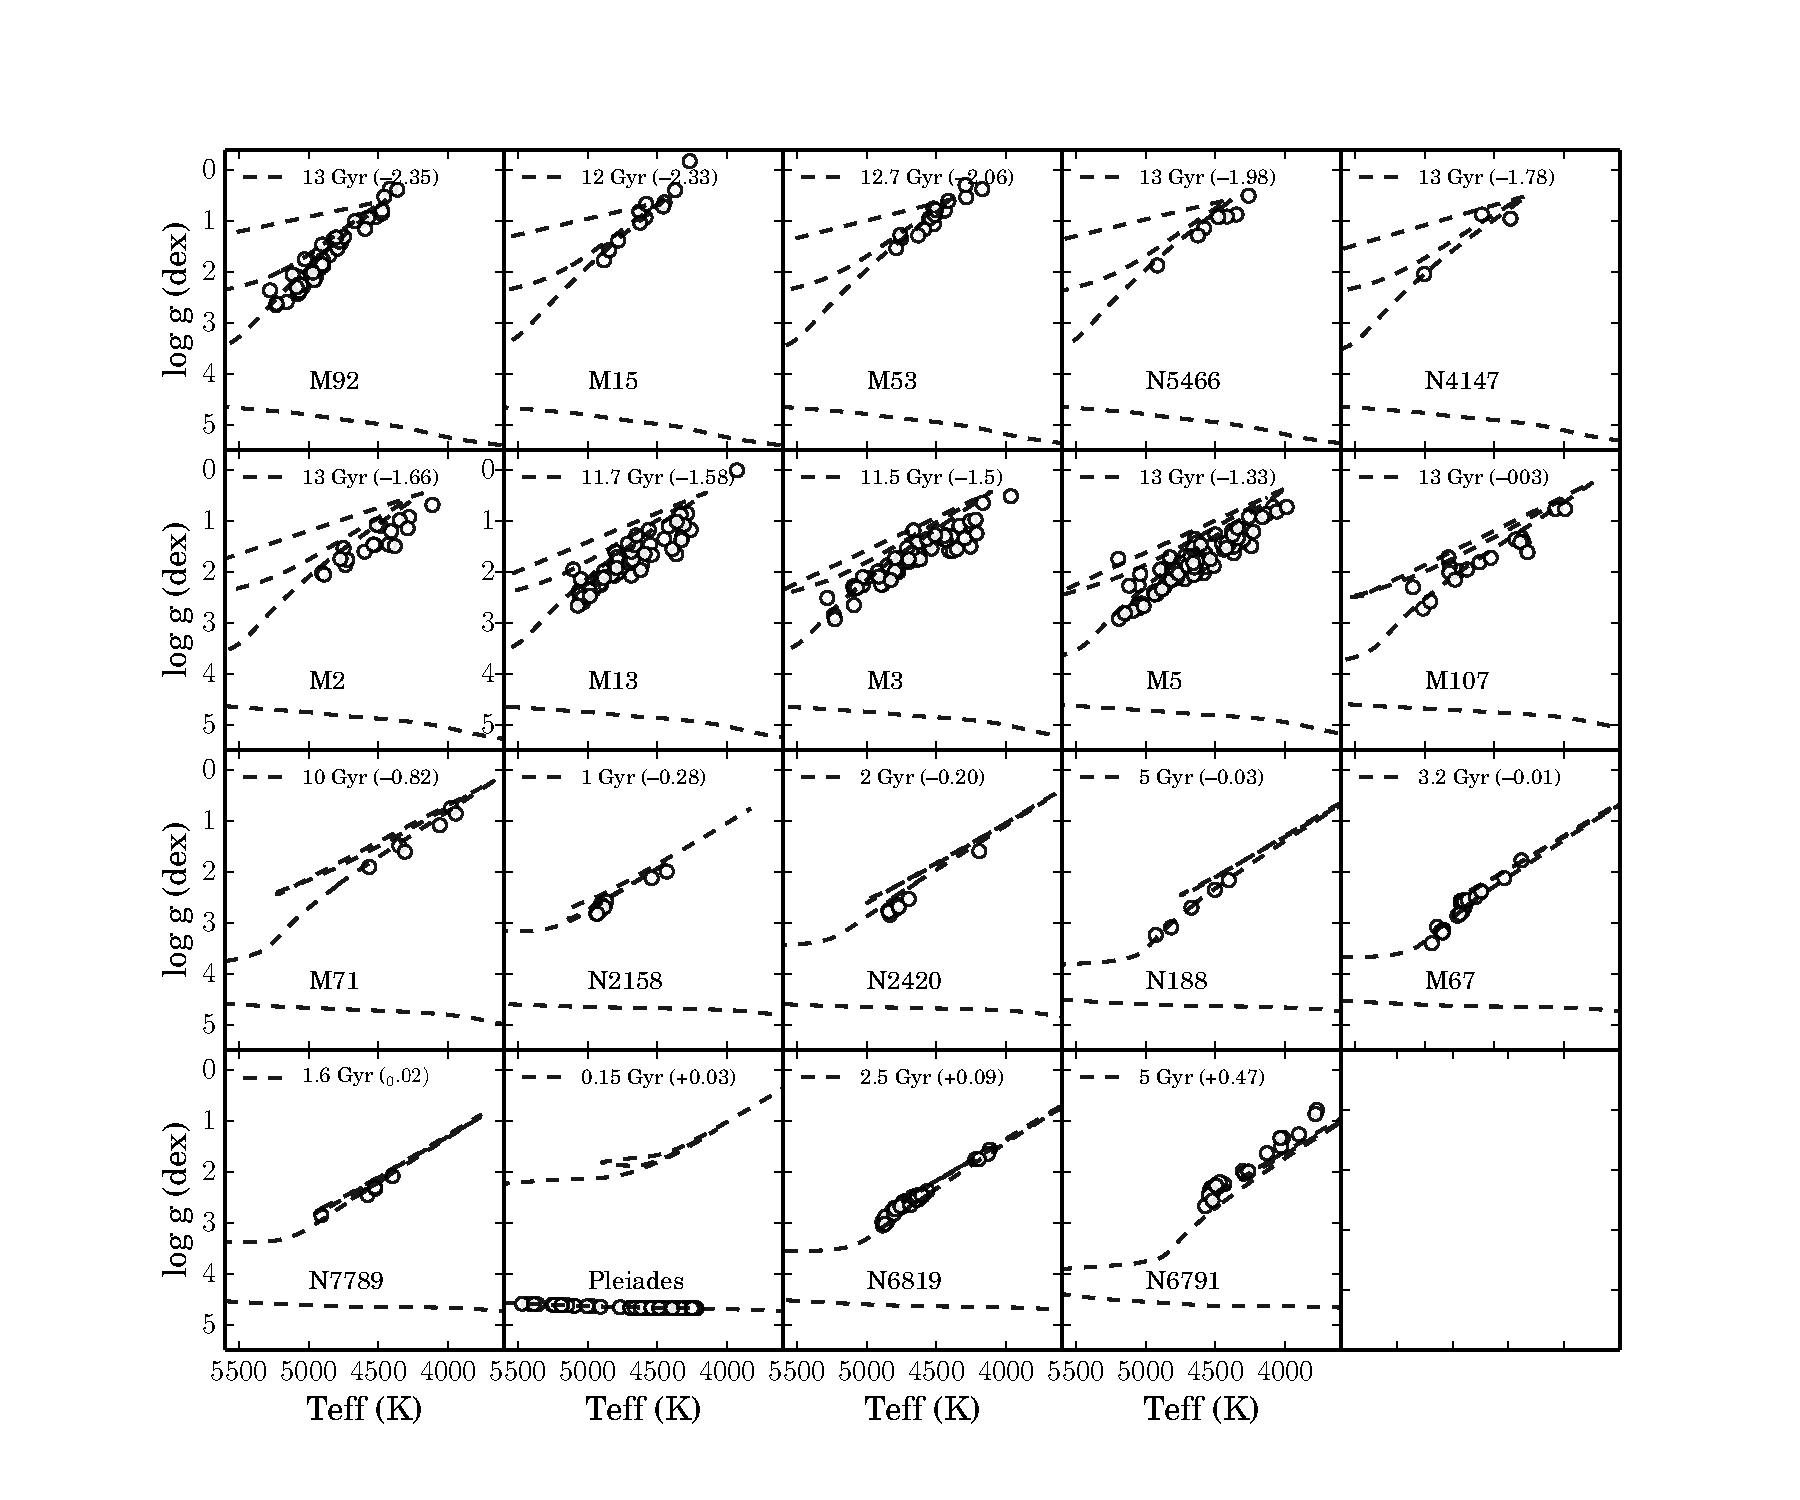
\includegraphics[scale=0.33]{./plots/training_aspcap.pdf}
\caption{\aspcap\ corrected training labels. All labels adopted from DR10 except for the Pleiades. }
\label{fig:trainingaspcap}
\end{figure}

\begin{figure}[h!]
\centering
  \includegraphics[scale=0.33]{./plots/training_mkn.pdf}
\caption{Isochrone-corrected \logg\ training labels: \teff\ and \feh\ labels are adopted from \aspcap-corrected results and the \logg\ labels are taken from vertical shifts to the isochrone. }
\label{fig:trainingisochrone}
\end{figure}


In the following sections we demonstrate that \tc\ reproduces \apogee\ \teff, \logg\ and \feh\ using a number of selected fields across the bulge, disk and halo with very small intrinsic errors which are comparable to \aspcap\ intrinsic errors at lower SNR than minimisation techniques. We provide an online table with the full set of parameters for \tc\ run through the APOGEE DR10 data comprising 51,500 stars in 170 fields that were available for download through the server at the time of writing this paper (some commissioning fields are not included).  We show all the stars run through \tc\ in the \teff-\logg\ plane comparing both calibration regimes and validate our method at low SNR.

%makeonisochrone_training_4panel.py




\section{Spectral Model}
\label{sec:spectralmodel}

The model is that the observed, continuum-normalized spectrum, at each
wavelength, can be explained as a linear combination of real-valued
``labels'', or a linear combination of functions of those labels.
Here the labels will be things like effective temperature $\teff$,
logarithmic surface gravity $\logg$, and metallicity $\feh$.
Additionally, the model is that at each wavelength, the observed
spectrum will deviate from the linear combination by some additive
noise contribution, some of which comes from photon noise and
sky-subtraction noise and other instrumental contributions, and some
of which is an intrinsic scatter, presumed independent at each
wavelength.
The model is built using ``training data'' (with known labels) and then
used to tag (or infer labels for) the ``test data''.

In the training data there will be $N$ spectra $n$, each of which has
a continuum-normalized flux measurement $f_{n\lambda}$ at wavelength
$\lambda$. Each of the training spectra $n$ has $K$ labels $\boldsymbol{l_{nk}}$, each of which
is (for now) presumed to have negligible uncertainty and contained within a label vector $\boldsymbol{x_n}$.

The general model is
\begin{eqnarray}
f_{n\lambda} &=&
\boldsymbol{\theta_\lambda}^T \cdot \boldsymbol{x_n} + \mbox{noise}
\
\end{eqnarray}

Where the flux $f_{n\lambda}$ of each spectra at every pixel is a general function of the labels which predict the spectrum given some noise, where $\boldsymbol{x_n}$ is some (possibly complicated) function of the full set of $K$ labels, $\set{l}_n$, which is is a vector or blob of the $K$ labels for spectrum $n$ and $\set{\theta}_\lambda$ is the set of parameters controlling the function $\boldsymbol{x_n}$ that determines the flux, at each wavelength.
%%

The simplest spectral model is that in which the function $\boldsymbol{x_n}$ is
linear in the labels, so this label vector is described as:
\begin{eqnarray}
\set{x_n} =  [1, l_1 - \bar{l}_1, l_2 - \bar{l_2}, l_k - \bar{l_k}, .. ] &\equiv& [l_{n1}, l_{n2}, \cdots, l_{nK}]
\end{eqnarray}.

The $\mean{l_k}$ are offsets (possibly means of the training data) to keep the model ``pivoting'' around a reasonable point in tag space.


Our general model then becomes
\begin{eqnarray}
f_{n\lambda} &=&
g(\boldsymbol{l_n} |  \boldsymbol{\theta_n}) + \mbox{noise}
\label{eq:linear}
\end{eqnarray}

Where the noise is a rms combination of the associated uncertainty variance
$\sigma_{n\lambda}^2$ of each of the pixels of the flux from finite photon counts and instrumental effects and the intrinsic variance or scatter of the model at each wavelength of the fit, $s_\lambda^2$. We assumed that the noise is Gaussian, zero mean, and independent for every measurement and the noise model is $\mbox{noise} = [s_\lambda^2+ \sigma_{n\lambda}^2]\xi_{n\lambda}$, where $\xi_{n\lambda}$ is a Gaussian random number with zero mean and unit
variance.

If there are missing flux values in the training data, these can be
handled by setting variances to something very large (or inverse
variances to something very small).

This model leads to the single-pixel log-likelihood function 
\begin{eqnarray}
\ln p(f_{n\lambda}\given\set{\theta^T}_\lambda, \boldsymbol{x_n}, s_\lambda^2) &=&
 -\frac{1}{2}\frac{[f_{n\lambda} - \set{\theta}_\lambda \cdot \set{x_n}]^2}{s_\lambda^2 + \sigma_{n\lambda}^2}
\label{eq:like}\\
\quad.
\end{eqnarray}


The vector $\set{f}_\lambda$ is the set of spectral flux values for
the $N$ objects all at wavelengths $\lambda$.
We can set the parameters $[\set{\theta}_\lambda,s_\lambda^2]$ either by
optimizing the likelihood (\ref{eq:like}) or by applying priors and
performing some kind of probabilistic inference (with, say, Markov
Chain Monte Carlo techniques).
Here we will optimize for now.

In this \sectionname, we are treating the function parameters
$\set{\theta}_\lambda$ and the scatter $s_\lambda^2$ as free parameters, and the
labels in the label vector $\set{x_n}$, $l_{nk}$ as fixed.
The likelihood function (\ref{eq:like}) is presented as being a
function of these free parameters.
In the next \sectionname, the tables will turn, and we will treat the
function parameters $\set{\theta}_\lambda$ and scatter $s_{\lambda}^2$ as fixed and
the labels $l_{nk}$ in the label vector, $\set{x_n}$, as parameters.
The difference is that here we are treating the training data as
having perfectly known labels, and later we will be inferring labels for
new spectra.

Then, in training, we determine:

\begin{eqnarray}
\set{\theta_\lambda} \leftarrow \substack{\mbox{argmax}\\
{\theta_\lambda}  }
\sum_{n=1}^N \mbox{ln p}(\set{f_\lambda} | {\theta_1,...\theta_\lambda})
\end{eqnarray}

The linear-in-labels form (\ref{eq:linear}) has many useful and
excellent properties.
The first is that optimization of the model, at fixed scatter
$s_\lambda^2$ is a pure linear-algebra operation (weighted least
squares); simultaneous optimization of all the parameters
$[\set{\theta}_\lambda,s_\lambda^2]$ is only nonlinear in the $s_\lambda^2$
parameter.

%
The second is that the tag inference (label-transfer; described in the
next Section) on the test data will have a very simple form.
The third is that the coefficients $\theta_{\lambda 0}$, seen as a discrete
function of wavelength $\lambda$, can be seen as an estimate of
the \emph{mean spectrum} (provided that the offsets $\mean{l_k}$ are
the mean tag values over the $N$ training spectra); and the
coefficients $\theta_{\lambda k}$ can be seen as the mean first derivatives of
the expected spectrum with respect to each of the $k$ labels, estimated
over the range of the training data.

The (perhaps) second-simplest spectral model is that in which the
functions $\set{x_n}$ are quadratic in the labels: so this label vector is described as:
\begin{eqnarray}
\set{x_n} =  [1, l_1 - \bar{l}_1, l_2 - \bar{l_2}, l_k - \bar{l_k}, (l_1 - \bar{l_1})(l_1 - \bar{l_1}), .. ] &\equiv& [l_{n1}, l_{n2}, \cdots, l_{nK}]
\end{eqnarray}.

This quadratic-in-labels form (\ref{eq:quadratic}) is similar to and
different from the linear-in-labels form (\ref{eq:linear}) in a number
of ways.
It is still the case that optimization of the model, at fixed scatter
$s_\lambda^2$ is a pure linear-algebra operation (weighted least
squares).
However, tag inference (described in the next Section) on the test
data will no longer be simple; it will now require non-linear
optimization.

The coefficients $\theta_{\lambda 0}$ can still be seen as an estimate of the
\emph{mean spectrum} (provided that the offsets $\mean{l_k}$ are the
mean tag values); the first-order coefficients $\theta_{\lambda k}$ can still
be seen as first derivatives of the expected spectrum with respect to
each of the $k$ labels, but now evaluated at the mean spectrum; the
second-order coefficients $\theta_{\lambda kk'}$ can now be seen as mean
second derivatives of the expected spectrum with respect to pairs of
labels $k$ and $k'$



\section{Parameter estimation}
\label{sec:paramestimate}

In the previous \sectionname, we built data-driven spectral models
from training data.
These models have the property that, given labels, they can be used to
predict continuum-normalized flux, up to observational and intrinsic
scatter.
In this \sectionname, we are going to solve the inverse problem; we
are going to presume that we have spectra, but we don't have labels.
In this case, we will use inference to obtain labels for the untagged
spectra.
These untagged spectra will be referred to as the ``test data'' in
what follows.

In the test data there will be $M$ spectra $m$, each of which---as in
the training data---has a continuum-normalized flux measurement
$y_{m\lambda}$ at each wavelength $\lambda$, and an
associated observational uncertainty variance $\sigma_{m\lambda}^2$.
Again, if there are missing flux values in the test data, these can be
handled by setting variances to something very large.
The difference between the training data and the test data is that the
test data do not (yet) have known labels $x_{mk}$; we are going to infer
these.

Just as in the previous \sectionname, our model is given in
equation~(\ref{eq:model}).
This model leads to the same likelihood function given in
equations~(\ref{eq:like1}) and (\ref{eq:like}), but this time seen as
being functions not of the function parameters $\set{\theta}_\lambda$ and
scatter $s_\lambda^2$ but instead as functions of the \emph{labels}
Then, in determining labels, we determine: 

\begin{eqnarray}
\set{l_\lambda} \leftarrow \substack{\mbox{argmax}\\
{l_n}  }
\sum_{\lambda=1}^\Lambda \mbox{ln p}(\set{f_\lambda} | {\theta_1,...\theta_\lambda})
\end{eqnarray}

where the likelihood functions are given as a function of labels now,
the sum is now over the full set of wavelengths
$\lambda$, and the vector $\set{y}_m$ is the vector of fluxes from
spectrum $m$ for all wavelengths $\lambda$.
These likelihood functions effectively assume that the function
parameters $\set{\theta}_\lambda$ and scatters $s_\lambda^2$ are all known (from
the training data).
New labels $\theta_{mk}$ for object $m$ can be obtained either by maximizing
the likelihood function (\ref{eq:taglike}), or else by applying priors
and performing probabilistic inference.
Here we will optimize for now.

When we use the simple linear-in-labels form (\ref{eq:linear}) for the
mean model $\set{x_n}$, the optimization to obtain maximum-likelihood labels
(given parameters $[\set{\theta}_\lambda, s_\lambda^2]$) is simple linear
least-square fitting.
This optimization is obtained by straightforward linear algebra on the
spectral pixels $y_{m\lambda}$, and standard frequentist confidence
intervals can be obtained similarly.

When we use the quadratic-in-labels form (\ref{eq:quadratic}) for the
mean model $Y()$, there is no simple linear-algebra operation that
optimizes the likelihood. Instead a python curve$\_$fit optimising function is used, which optimises the values for the parameters so that the sum of the squared error of f(xdata, $*$popt) $-$ ydata,  is minimized. 

We have described how we construct our model and then apply our model to get labels for new stars, We now present in \ref{sec:results} the results for our model, starting with the simplest linear first-order implementation and then for the model we used for all \apogee\ data, of the quadratic model, linear in the coefficients and non-linear in the label-inference.  For the quadratic model we then show this applied to the DR10 data, including at lower SNR and investigate different input training labels. 



\section{Results}
\label{sec:results}

We have five primary results from the implementation and running of \tc\ through the DR10 \apogee\ dataset. The first is that we can demonstrate, via the scatter of the fit, that our model is a good fit to the data. This says that our model is predictive and we perform a cross validation to assess the errors we expect for our test data, which is the DR10 \apogee\ spectra. A cross validation performed with a take-one-cluster out test however tells us that our training sample is too small, each cluster is critical to the results. It is clear from our results that we are also critically lacking in dwarf training spectra. If the Pleiades stars, which comprise the dwarfs, are removed we can not recover parameters for dwarfs and so can not differentiate dwarfs in the test data.
Via our method, we can use the model for determining continuum pixels, which are robust and true continuum over the label-space of the training data. This continuum normalisation is a key second result and we implement this for both training and test data and validate it is robust across SNR. 

This success of the method using the DR10 data is our third result.  Despite of the critically constrained training set for our model, the label-transfer method using DR10 test data works extremely well. This showcases the strength in this approach, that with only 550 training stars, we can reproduce all DR10 labels for the stars in the \apogee\ survey, quickly and simply.  
We reproduce the \aspcap\ DR10 labels, of \teff\, \logg\ and \feh\ with errors of \teff\ $<$ 100 K, \logg\ $<$ 0.20 dex and \feh\ $<$ 0.10 dex. The rms dispersion of \apogee\ -- \tc\ is no larger than \apogee\ parameter errors reported in \citep{Meszaros} as our method generates insignificant errors at the SNR of the combined visit \apogee\ data. We also report results for dwarfs but these are constrained by the very limited dwarf set in our training sample, and we do not provide a robust measurement of these stars across metallicity, given our single metallicity dwarf training set.

The fourth result, from the testing of the DR10 data is that objects which are not in our training data set give unphysical parameters in their labels. These objects with unphysical parameters were found to be fast rotators, which can be easily excluded using the \aspcap\ rotation warning set flag. This demonstrates that we can only be as good as our training set. 

The final result that we report is the performance of \tc\ at low SNR. We demonstrate that \tc\ returns robust stellar parameters at an SNR of $<$ 30. For this test we do not nosify the spectra but rather use the single visit spectra available in the \textit{apStar} DR10 data files. The performance of \tc\ at low SNR reflects both the success of the continuum identification and the strength in using \textit{all} of the spectral range to characterise the labels by allowing the regression to determine which pixels control the labels themselves.


\subsection{The model} 

To firstly evaluate the label-transfer method, we performed the simplest implementation of a first-order linear model comprised of four coefficients. Figure \ref{fig:self1} shows the performance of this model for the 550 stars in the training set, run back through \tc\, having used the very same stars to set the coefficients for the model. The bias, rms and precision represent the offset and difference between the input and output labels and the internal error of the label inference, respectively.  The first -order linear model is clearly too inflexible to describe the behaviour of flux with the labels. This is not surprising given it is known that absorption features and particularly strong lines, do not behave linearly to the first-order, as a function of stellar parameters. Different metallicity regimes show different trends in  temperature and \logg\ and the dwarf labels are not well reproduced, showing large scatters in the \logg\ and \feh\ labels. 

The linear model can be vastly improved by selecting only weak line regions, and excluding all strong lines by implementing a cut on the normalised flux considered for the coefficients fit in the label-transfer. The loss of information in the exclusion of a significant fraction of pixels is however clearly subtimal. 

% run -i takeoneoutplot_all_comparison_singleorder.py
\begin{figure}[h!]
\centering
  \includegraphics[scale=0.45]{./plots/single_self.pdf}
\caption{The performance of the label-transfer of \tc\, where input coefficients have been determined using the set of training stars then run back through \tc\ as test data, to determine how the model can predict their labels; a test of the ``goodness'' of the model, for the simplest linear case with four coefficients. }
\label{fig:self1}
\end{figure}

The perhaps the second simplest model we can implement, is the quadratic model, with ten coefficients describing the labels, (\ref{eq:linear}).  Overall, this model describes the behaviour of the flux with the labels across their parameter space fairly well and is clearly significantly better than the first-order linear model within the parameter range of these stars. 

The results for the first-order coefficients and the scatter of the fit for the quadratic-in-labels model, is shown in Figure \ref{fig:coeffs}, across the narrow regions (a) and (b) of the spectra, marked in Figure 1. The top panel shows the scatter of the fit, indicating the dispersion of the flux of the training data around the model at each pixel and the mid-panel corresponds to the intersect of the model of the training sample, with regions of first order label dependence shaded in the different colours corresponding to \teff, \logg\ and \feh. The bottom panel shows the first order coefficients $\theta$ in \teff, \logg\ and \feh.  The scatter is small and this indicates that our model is a good representation of the data. From this intersect flux, the continuum pixels have been determined, which  are then used for the final continuum normalisation for the stars, both training data and test data. 

 In the mid-panel of Figure \ref{fig:coeffs}, the red, blue and green shaded regions show the highest 2$-\sigma$ coefficient values $\theta_{1,2,3}$ in the \feh, \teff\ and \logg\ labels respectively, shown in the bottom panel of the Figure. These regions indicate where these flux levels are strongly proportional to these labels and highlights the differences between the labels in their flux dependancy. Note there are many regions where the \feh\ label dominates in contribution to the flux. From the bottom panel of Figure \ref{fig:coeffs}, it is clear that there is significant covariance between the labels and the \logg\ label has the weakest first-order dependence on the flux of the three labels across this sample wavelength interval. 

By returning coefficients, we have a tool which describes the flux in a quantitative way as a function of stellar labels, thus removing degeneracies and improving the prospects for determining stellar parameters, by modelling covariance rather than attempting to minimise it. 

For the overall label profiles in the middle panel of Figure \ref{fig:coeffs}, there is typically asymmetry for a given absorption feature, in the flux and the labels. There are very few regions were the flux is a function of only one of the labels, and pixels are typically covariant. The strongest \logg\ dependence is typically associated with weak lines and the \teff\ and \feh\ labels, with strong lines. 

 
 %made with run -i makeplot_scatter_test18_step.py
\begin{figure}[h!]
\centering
    \includegraphics[width=\hsize]{./plots/R1_continuum2.pdf}
  \caption{Top panel: the scatter of the fit, middle panel: the mean spectra from the first coefficient, from the training set and the bottom panel; the first three coefficients ($\theta_1$, $\theta_2$, $\theta_3$),  which correspond to the first-order label terms ($\teff, \log, \feh$).   The red, blue and green shaded regions show the highest 2$-\sigma$ coefficient values in the \feh, \teff\ and \logg\ labels respectively. This indicates where these flux levels are strongly proportional to the labels. Note the \feh\ label is dominant in the contribution level and from the bottom panel it is clear that there is significant covariance between the labels and lesser regions of strong \logg\ dependence, across this sample wavelength interval.}
\label{fig:coeffs}
\end{figure}

To assess the uncertainty of our model, we perform a take-one-cluster out test and a take-one-star out test. This is a conservative way to check our expected error bars on our test data given our model. For the take-one-cluster out test we train the model iteratively on all clusters except for an excluded one, and then run the removed cluster through the label-transfer, to see how well the model can predict labels for the cluster stars. Similarly, for individual stars.  

Figure \ref{fig:takeoneout} shows the cross-validation results for take-one-cluster out test. This Figure demonstrates that each cluster is critical to the training set and removing even one is extremely detrimental to the model. This is the most conservative test we can implement to assess the error bars expected from our model and the clear sensitivity indicates that he model is significantly too small and certainly sub-optimal. We can only do better by expanding on this most basic model. Additionally, for the take-one-cluster out test, if the training set does not include the cluster with dwarfs, the Pleiades, then these stars are not recognised as dwarf stars. This set of dwarf training data is therefore essential to recognise dwarfs and discriminate them from giants, which is important in our running through all of the DR10 spectra. There are limitations however in this dwarf discrimination, in that not all spectral types observed as part of DR10, namely hot dwarfs with rotation, are included in our model and we can discriminate these stars based on their returned labels, but can not return correct labels for these stars. 

\begin{figure}[h!]
\centering
  \includegraphics[scale=0.45]{./plots/quad_takeoneout.pdf}
\caption{Take-one-cluster-out cross validation}
\label{fig:takeoneout}
\end{figure}

Figure \ref{fig:takeonestarout} shows the cross-validation results for take-one star out. The results for the bias and rms are indicative of how well our model performs over the full , and these will inherently include the uncertainties on the input labels (from ASCPAP corrected values, of \teff $<$ 150 K, \logg $<$ 0.2 dex and \feh\ $<$ 0.1 dex \citep{Meszaros2013}. There are outliers, and certain cluster members, M3 and M5 and stars in M13 in particular, seem grouped together, offset in \teff\ and \logg\ space. Removing these clusters improves the rms in the \teff\ and \logg\ labels by 10\%. The single dwarf cluster shows the poorest determination in the \feh\ label and this cluster was set at a single metallicity, dissimilarly to the other training data which used \aspcap\ corrected parameters which were provided. The rms is comparable and less than the estimated \apogee\ errors with \logg\ performing the most over the \apogee\ estimates.  

The outlying stars in Figure \ref{fig:takeonestarout} may be due to an anomalous scale of the input labels of these stars compared to the other training data, or it may be due the nature of the spectra of these stars, that is not accounted for in the model. Similarly, the temperature of the dwarfs is offset low at increasing temperature, compared to the input labels, so the model may be limited in describing the difference between dwarf and giant spectra. The labels perform best in \feh\ space, which may not be surprising given the information content in the [Fe/H] coefficient seen in Figure \ref{fig:coeffs}. However, there is a flattening at the low metallicity end of the model in \feh\ in the output labels at \feh\ $<$ -2.2. 



\begin{figure}[h!]
\centering
  \includegraphics[scale=0.45]{./plots/takeonestarout.pdf}
\caption{Take-one-star-out cross-validation}
\label{fig:takeonestarout}
\end{figure}


\subsection{Continuum identification}



These continuum pixels have been determined from the quadratic model using a combination of the flux level and the coefficients returned.  From the intersect-flux returned in the first coefficient, 35\% of the pixels across this wavelength region have a pixel level within 1\% of flux = 1. However, regions where the intersect-flux is $\sim$ 1 are not representative of continuum for all stars in the training set, e.g. metal rich stars. It is insufficient to select on pixels that are simply near the intersect-flux in isolating continuum regions. Instead, we are informed by the coefficients of the fit. A set of coefficients which are near 0, is indicative of a pixel region where there is no dependence, or negligible dependence of the flux on the labels, across all of the training spectra. We make a final continuum selection taking the 15\% of pixels with coefficients nearest 0, for each coefficient and a flux selection of 1 $\pm$ 0.15. This criteria returns around  7\% of pixels, which we adopt as true continuum pixels for data that spans the parameter range of the training set. We use the inverse variance weighting of these pixels for the corresponding Chebyshev fit which we find to be a robust continuum normalisation across the stars that are within the parameter range of the training set, across all SNR. The continuum pixels are marked on sample spectra from the training data, across the metallicity regime of most metal-poor to most metal-rich cluster in Figure \ref{fig:cal_feh}.


% made with  makeplot_scatter_test18_coeffs.py
\begin{figure}[h!]
  \includegraphics[width=\hsize]{./plots/3training.pdf}
\caption{Three stars from the training data: top M92 (\teff\ = 4995 K, \logg\ = 2.1 dex ,\feh\, = -2.2 dex) middle = M5 (\teff\ = 4302 K, \logg\ = 1.4 dex, \feh\ = --1.25 dex), bottom panel: N6791 (\teff\  = 4495 K, \logg\ = 2.3 dex, \feh\ = 0.4 dex. \textbf{Need to improve continuum normalisation so first panel does not look like first panel currently does}. }
\label{fig:cal_feh}
\end{figure}

\subsection{DR10 Comparison}

Using our model, which is clearly sub-optimal in its size and its diversity of spectra, we are nevertheless able to reproduce all of the \aspcap\ labels for DR10 spectra. We have run \tc\ through all (non-commissioning) stars in DR10 contained in the available \textit{aspcapstar} files,  which comprise about 46,800 stars, in 150 fields and an additional 4800 stars in 20 commissioning fields for which no \aspcap\ parameters were provided in DR10, made available in the (non pseudo-continuum normalised) \textit{apStar} files. These 170 fields comprise a total of $\sim$ 51,600 \apogee\ DR10 stars. 

The comparison of \tc\, showing the bias, rms and precision for 6 sample fields, with bulge, disk and halo targeting are provided in Figure \ref{fig:cal}. We reproduce the \aspcap\ corrected stellar parameters with typical rms uncertainties of \teff\ $<$ 100 K, \logg\ $<$ 0.20 dex and $<$ \feh\ $<$ 0.10. These errors are slightly better than the expectations provided with our cross-validation leave-one-star-out test which may be because the median of the test data stellar parameters are near the median labels of the training data and not concentrated to the extreme ends of the range, which have a higher weighting in evaluating the test data with cross validation. In addition, we also return a fraction of about 15\% dwarfs (not shown in these Figures as \apogee\ does not report ASCAP corrected dwarf parameters for DR10). We exclude the rapid rotators using the \aspcap\ \rotwarn\ flag as we can not return parameters for spectral types not included in our training set. 

\begin{table*}[!h]
\small{
\centering
\caption{Excerpt from full online version of table of parameters for the 51,500 stars released in 170 fields from APOGEE's data release DR10. Stars with rotation warning = 1 flag set have unphysical stellar parameters.} \begin{tabular}{| c | c | c |  c | c | c |  c | c | c |}
\hline
star ID & \teff\ & \logg\ & \feh\ & $\sigma$(\teff) & $\sigma$(\logg) & $\sigma$(\feh) & $\chi^2$ & \tiny{ROT WARN}\\
{2MASS} &  K &  dex  & dex & K & dex & dex & & \\    
\hline
%21353892+4229507 & 4131.7 &  1.51 & 0.04 & 3.25 & 0.0116 &  0.0042 & 11.06 &  0.0\\
21354474+4250256 & 5028.5 & 4.53 & 0.13 & 9.14 & 0.01 & 0.006 & 3.14 & 0\\
21354775+4233120 & 4730.9 & 2.8 & 0.06 & 12.02 & 0.04 & 0.011 & 1.34 & 0\\
21355458+4222326 & 4780.1 & 2.42 & --0.36 & 8.34 & 0.03 & 0.007 & 2.41 & 0\\
21360285+4231145 &  4552.4 &  1.96 & --0.46  & 10.83 & 0.04 & 0.011 &  1.42 &  0\\
 \hline
\end{tabular}
\label{tab:online} }
\end{table*}  
 
%makeplot_fits_v19_bw.py
\begin{figure}[!h]
\centering
  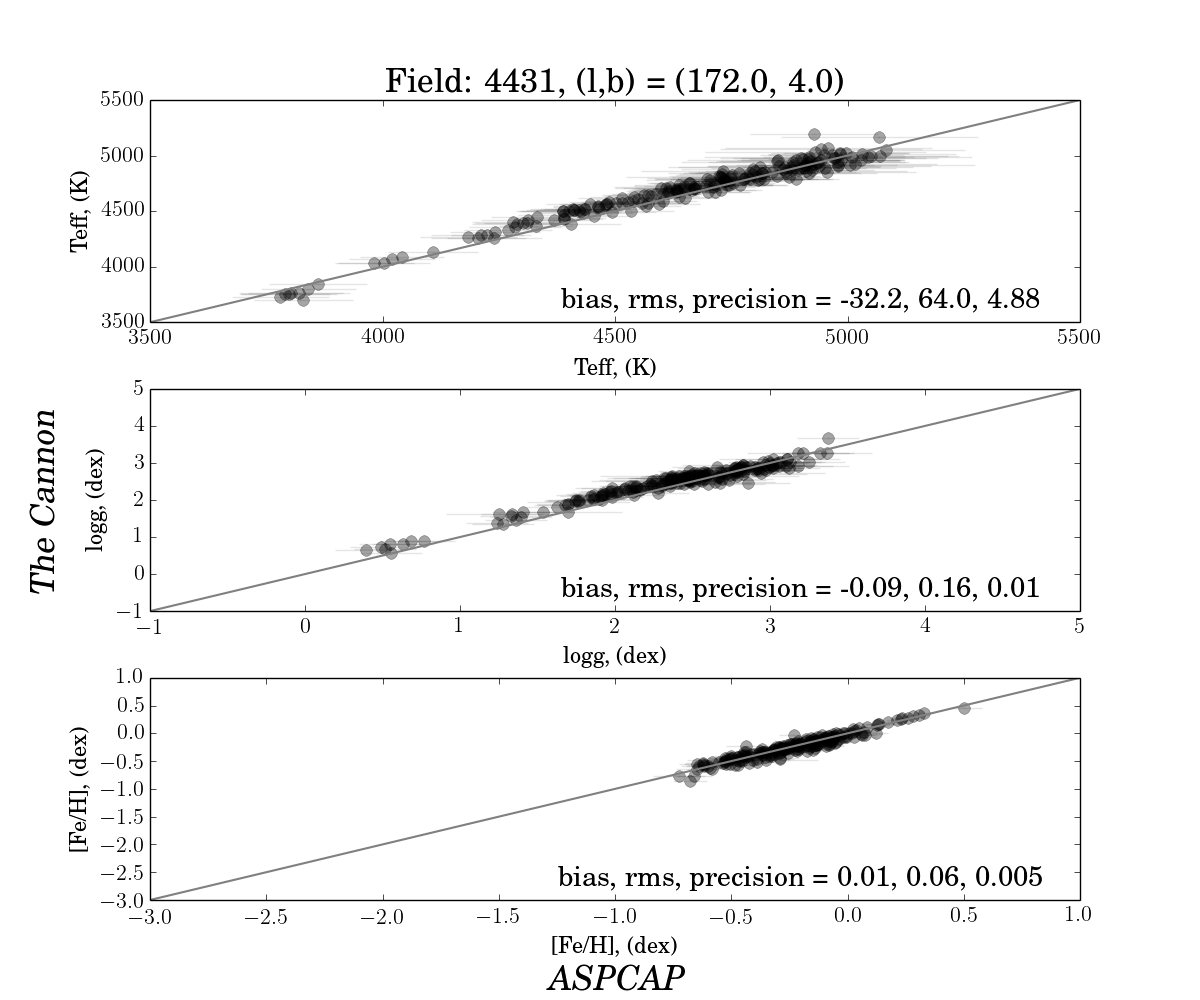
\includegraphics[scale=0.23]{./plots/4431_v19.pdf}
    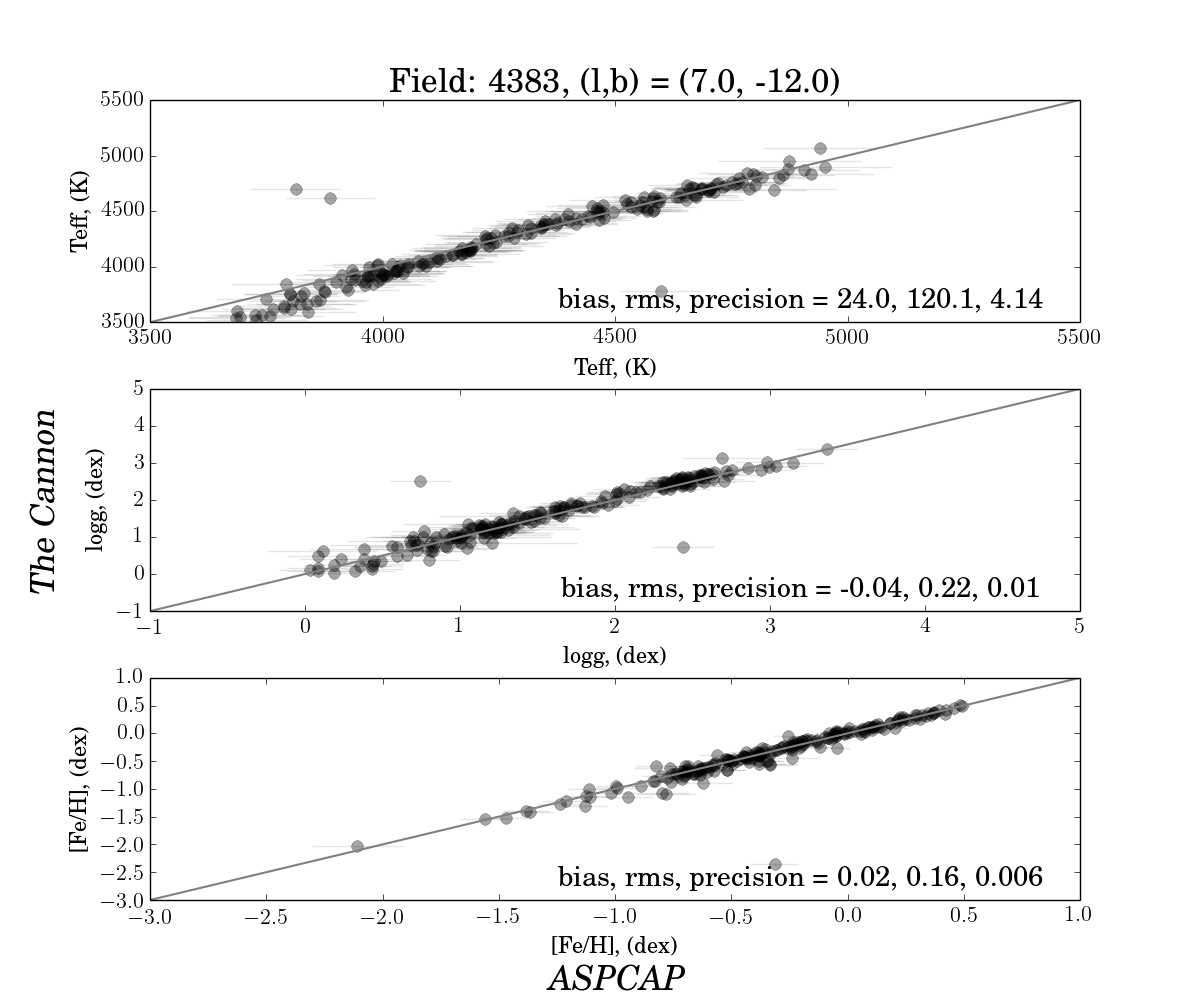
\includegraphics[scale=0.23]{./plots/4383_v19.pdf} \\
      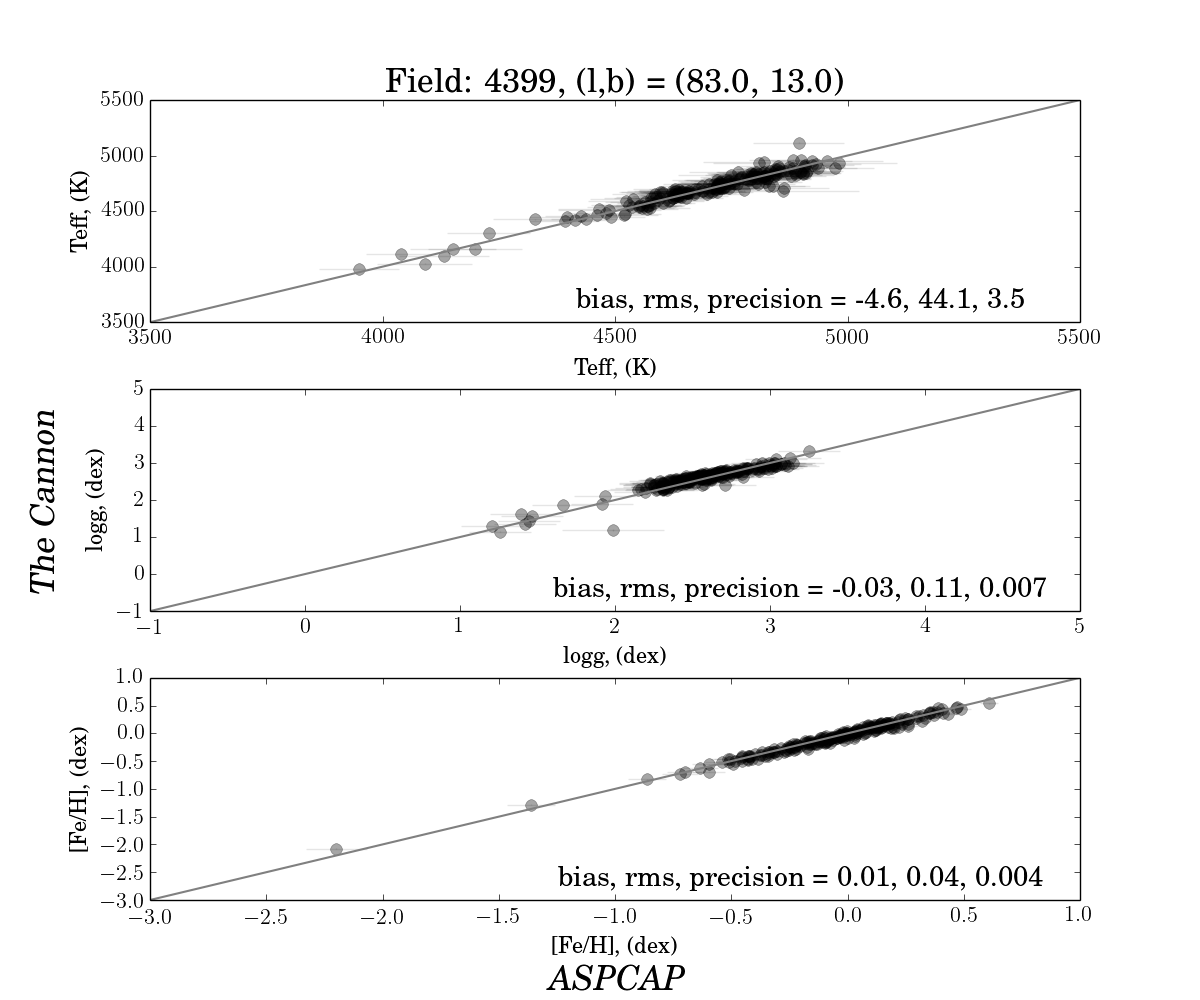
\includegraphics[scale=0.23]{./plots/4399_v19.pdf}
        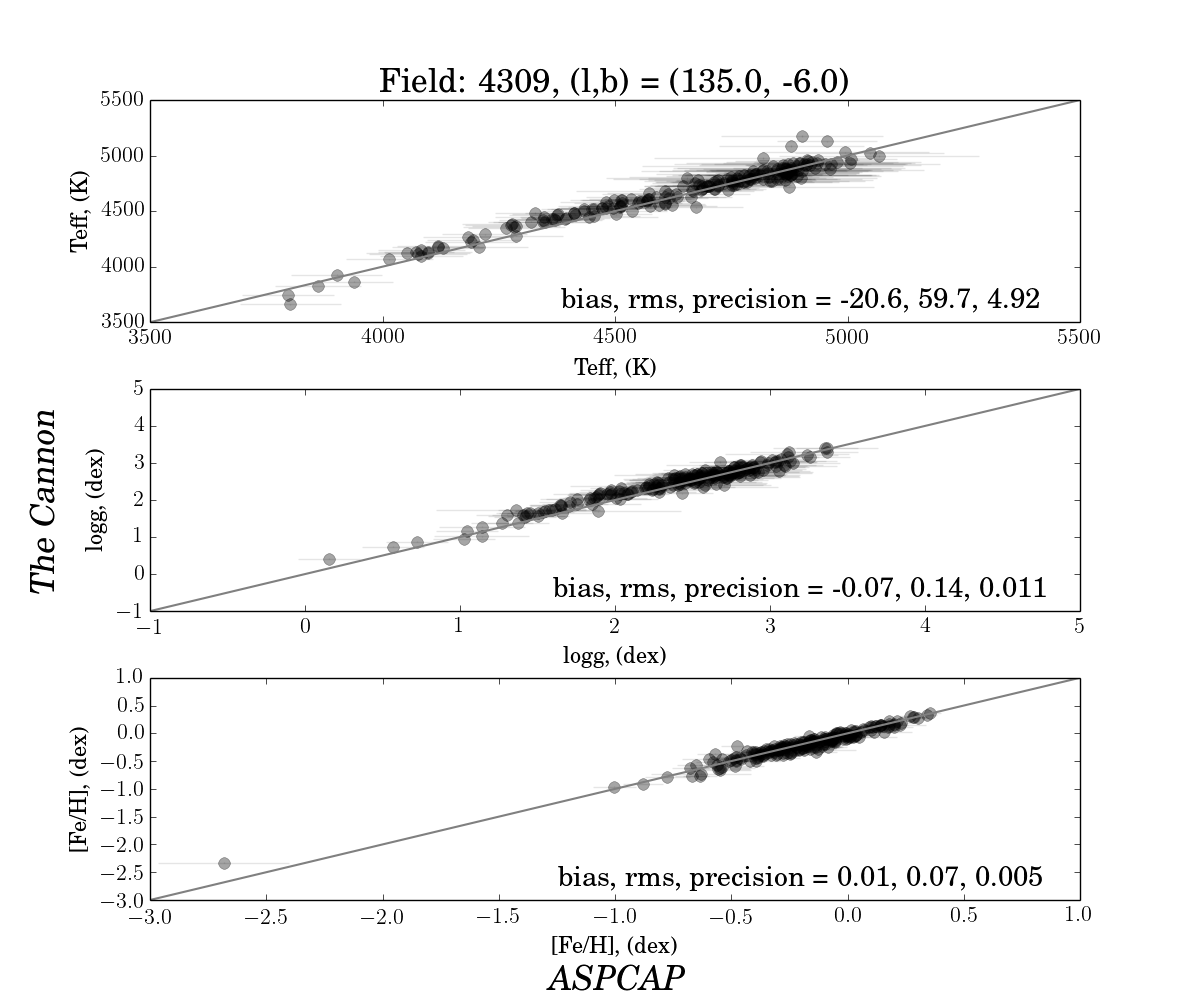
\includegraphics[scale=0.23]{./plots/4309_v19.pdf} \\
              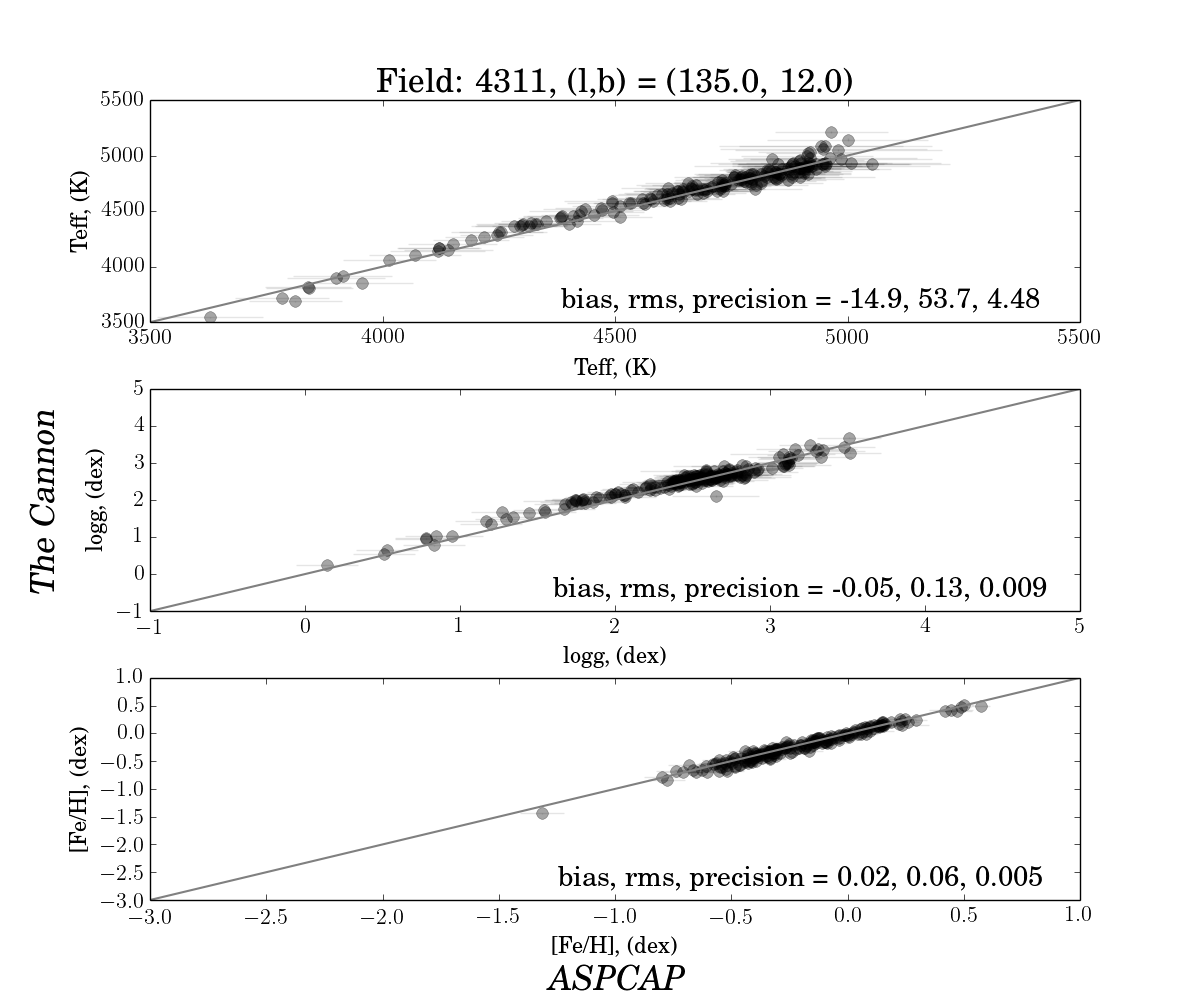
\includegraphics[scale=0.23]{./plots/4311_v19.pdf}
        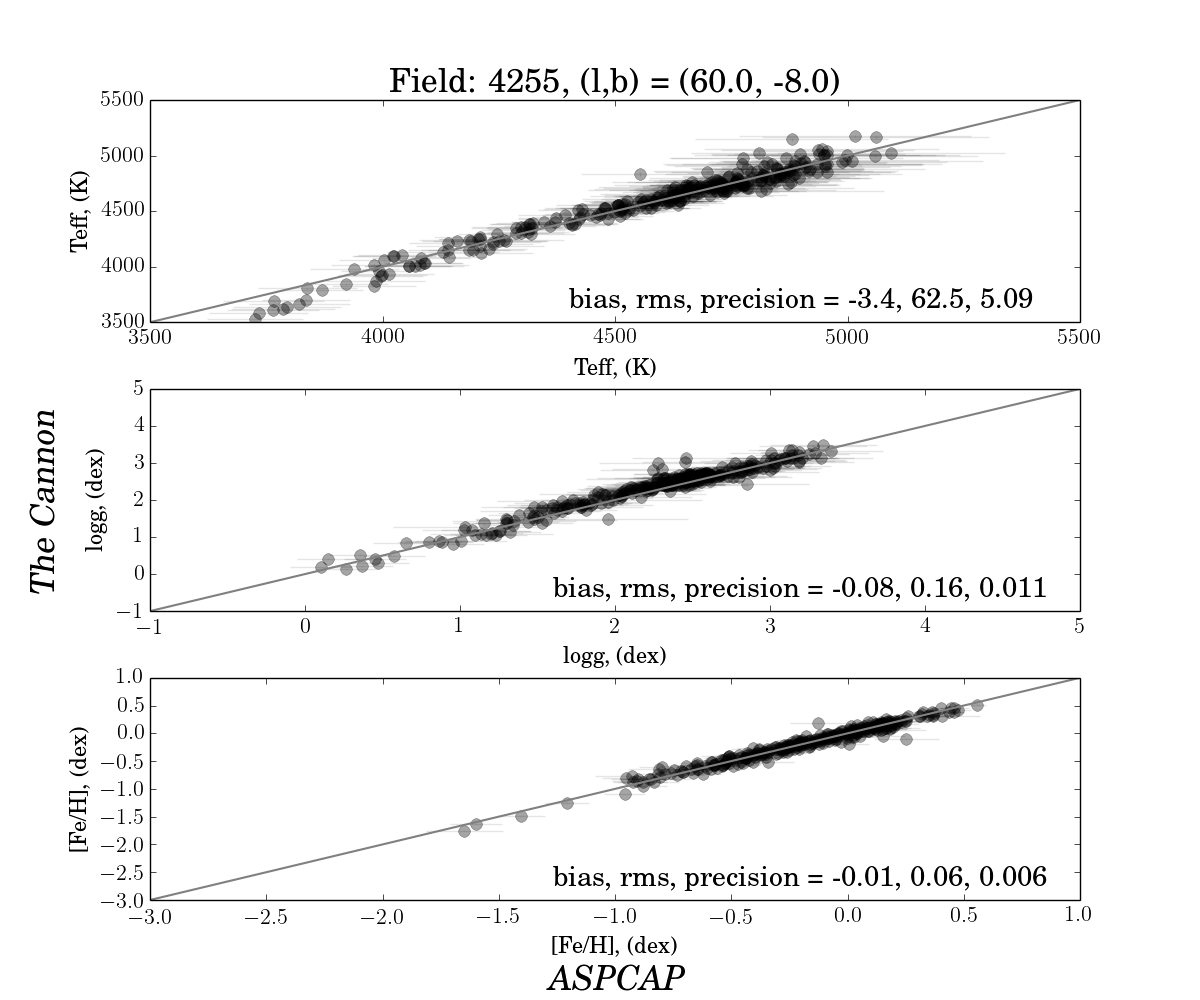
\includegraphics[scale=0.23]{./plots/4255_v19.pdf} 
\caption{\small{\aspcap\ DR10 versus \tc\ for 6 different fields including in the disk, bulge and halo. The number of stars is, for each subfigure is 211 (4431), 207 (4384), 217 (4399), 210 (4309), 198 (4311) 319 (4255) }}
\label{fig:cal}
\end{figure}

%run -i makeplot_fits_v19_3by3b.py
\begin{figure}[!h]
\centering
        \includegraphics[scale=0.35]{./plots/cplot.pdf} 
\caption{The \teff, \logg, and \feh\ trends for the 1400 stars shown in 6 different fields in Figure \ref{fig:cal}. There are slight trends at the extreme ends of the range in parameters.}
\label{fig:cplot}
\end{figure}

The results of \tc\ for all DR10 stars for which we return parameters is provided online in Table \ref{tab:online}. For the 30,500 stars with parameters provided by DR10, we find we reproduce the \apogee\ labels at \teff\ = +12 K $\pm$ 87 K ,  \logg\ = --0.04 dex $\pm$  0.18 dex and \feh\ = +0.01 $\pm$ 0.10 dex in \feh. The rms errors are comparable to the error estimates for \apogee\ parameters in \citet{Meszaros2013} of $\delta$(\teff) $<$ 150 K, $\delta$(\logg) $<$  0.2 dex and $\delta$(\feh) $<$  0.1 dex in.  The typical internal precision on the measured parameters from \tc\ is  $\delta$(\teff) $<$ 5.6 K in ,  $\delta$(\teff) $<$ 0.01 dex in \logg\ and  $\delta$(\teff) $<$ 0.006 dex in \feh.

We show the location of the stars in the \teff-\logg\ plane from \tc\ for the stars in DR10 in Figure \ref{fig:iso} where the top panel shows the training labels input directly from \aspcap\ corrected labels and the bottom panel shows the results for the isochrone-corrected labels. There are 37,500 stars in these Figures which are remain after excluding stars with the \rotwarn\ flag set, with velocity scatter $>$ 10 \kms\ and telluric calibration target set. For approximately 15\% of these stars, we return dwarf parameters for, with \logg $>$ 4 dex.  The stars that have been determined using targeting flags and inspection of the spectra, to be dwarfs with rotation, lie in an unphysical space at very low \feh\ and log g and have been removed using the \aspcap\ rotation warning set flag.
%From our total of  51,600 stars, then cut down to 39,500 after cutting out  the approximately 7500 stars with

Although we find excellent agreement between \tc\ and \aspcap\ by adopting ASCPAP corrected labels and additionally are able to derive parameters for dwarf stars in DR10, the \teff-\logg\ plane for these stars shows an unphysically narrow giant branch  (see the left panel of Figure \ref{fig:iso}). The narrowness of the giant branch is necessarily a consequence of the input labels of the training spectra. 

% made with makeonisochrone_v18_bw.py
\begin{figure}[!h]
\centering
  \vspace{-15pt}
  \includegraphics[scale=0.33]{./plots/isochrone_v19b.pdf}

    \includegraphics[scale=0.33]{./plots/isochrone_mkn20b.pdf}
\caption{The $\sim$ 37,500 stars from DR10 at top with the \aspcap-corrected training labels and at bottom with the ``isochrone-corrected'' \logg\ training labels, shown in four metallicity bins. Note the different \logg\ distribution at low \logg\ along the giant branch. There are $\sim$ 21,600, 14,000, 1700, and 900 stars in the most metal-rich to metal-poor metallicity bins, respectively. The isochrones plotted at 10 Gyr Padova isochrones at the metallicities marked in the upper left hand corners of each sub-panel.}
\label{fig:iso}
\end{figure}


The results using our isochrone-corrected \logg\ calibration (described in the Introduction) remove our results slightly from the \aspcap\ scale in each of the parameters. However, with these new \logg\ labels, we find a broad giant branch width that is consistent with expectations in \teff-\logg\ space given the metallicity of these stars (see the right hand panel of Figure \ref{fig:iso}).

%Using our own calibration of the \logg\ values, we also find good  good agreement with Kepler \logg\ values. The difference between Kepler and \tc\ \logg\ values is also \teff\ independent, which is not the case for training on the \apogee\ labels. 


%% made with 
%\begin{figure}[h!]
%  \includegraphics[width=\hsize]{./plots/isochrone_mkn20b.pdf}
%\caption{Training labels using own labels in \logg\ : moved to isochrone}
%\label{fig:mknA}
%\end{figure}


\subsection{Anomalous Spectra: Dwarfs and Rotation}

 
  \begin{figure}[!h]
   \centering
 \includegraphics[width=\hsize]{./plots/3dwarfs.pdf}
  \caption{Examples of hot rotating dwarfs in the \apogee\ DR10 data which are not included in our training data; we can not determine stellar parameters for these stars as they are not captured in our model.}
\label{fig:dwarfs}
\end{figure}


The dwarf spectra in our training set consists of the Pleiades cluster, at a single metallicity. This restricted sample constrains our ability to determine the stellar parameters for dwarf stars. Given these training data, our model \textit{can} differentiate dwarfs from giants, as long as their spectra is comparable to that of the Pleiades. However, none of the dwarfs in our training set are hot rotating objects, with broad line features, for example the stars in Figure \ref{fig:dwarfs}, which comprise a fraction of \apogee\ DR10 data. 

It is possible to differentiate these stars with \tc\, as they are output in non-physical space in \teff-\logg, and present as a group of very metal poor, \feh\ $\sim$ --2.0, low \logg\ stars $\sim$ 0, with cool temperatures $\sim$ 4000 K. The metal poor solution determined by \tc\ reflects the dearth of lines in the spectra for these hot stars, given the training model. 

This group of stars is flagged in \aspcap\ with a \rotwarn\ flag set. We therefore are able to exclude these stars from our analysis using this condition. 
 

 
 %  makeplot_scatter_test18_coeffs_dwarfs.py


 \subsection{Performance at low SNR}
 
 \begin{figure}[!h]
  \includegraphics[width=\hsize]{./plots/SNR_continuum.pdf}
  \caption{Demonstration of the continuum normalisation of the same star at high and low SNR. The \apogee\ reported SNR of the combined visit spectra is SNR = 120 (top two panels) and of the 4th visit shown in the third pane is 25 (bottom two panels) }
\label{fig:lowsnr}
\end{figure}

%makeplot_fits_SNRtest.py in /play but changed to makeplot_fits_SNRtest_bw.py
 \begin{figure}[!h]
 \centering
 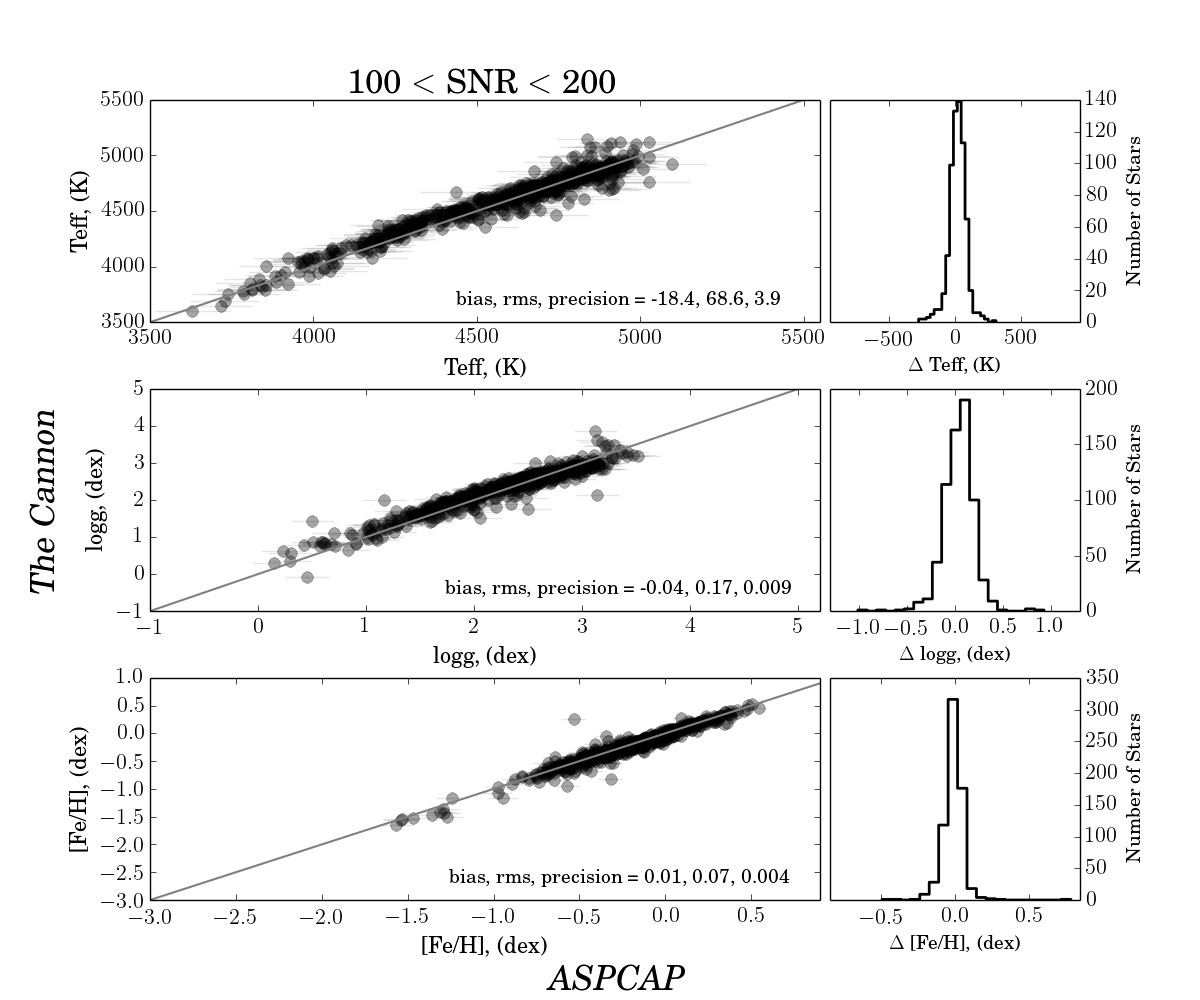
\includegraphics[scale=0.25]{./plots/SNR100to200.pdf}
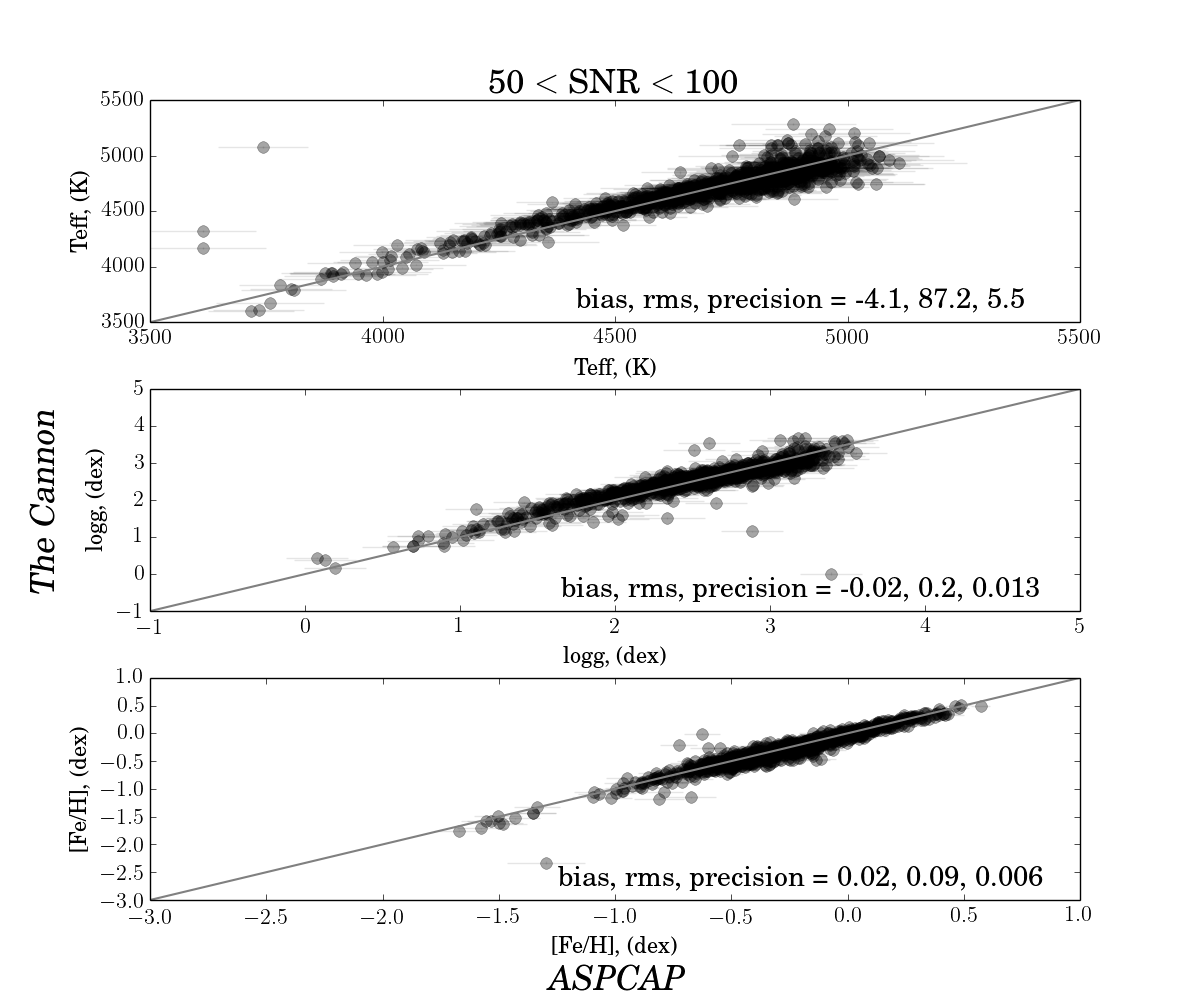
\includegraphics[scale=0.25]{./plots/SNR50to100.pdf}\\
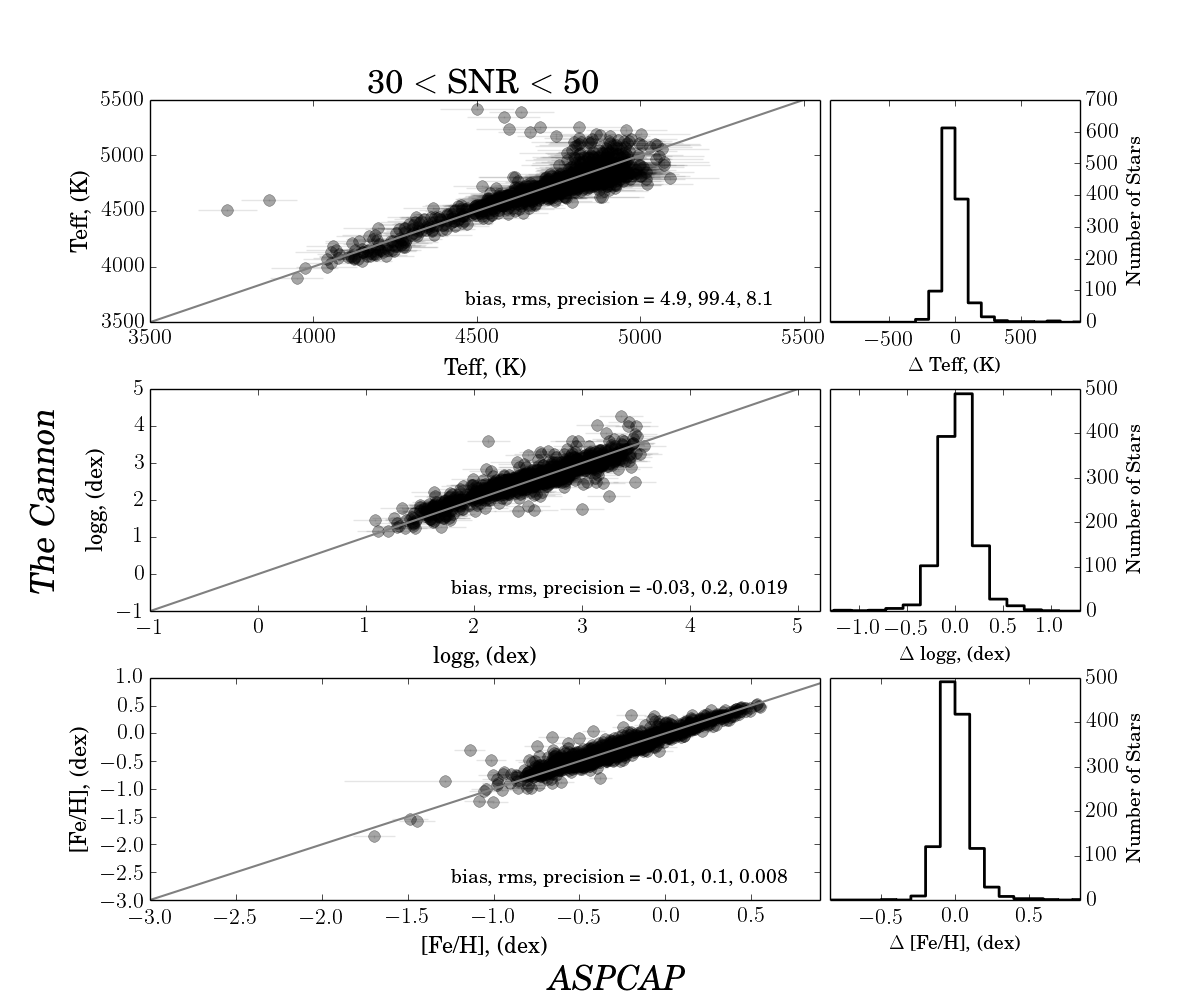
\includegraphics[scale=0.25]{./plots/SNR30to50.pdf}
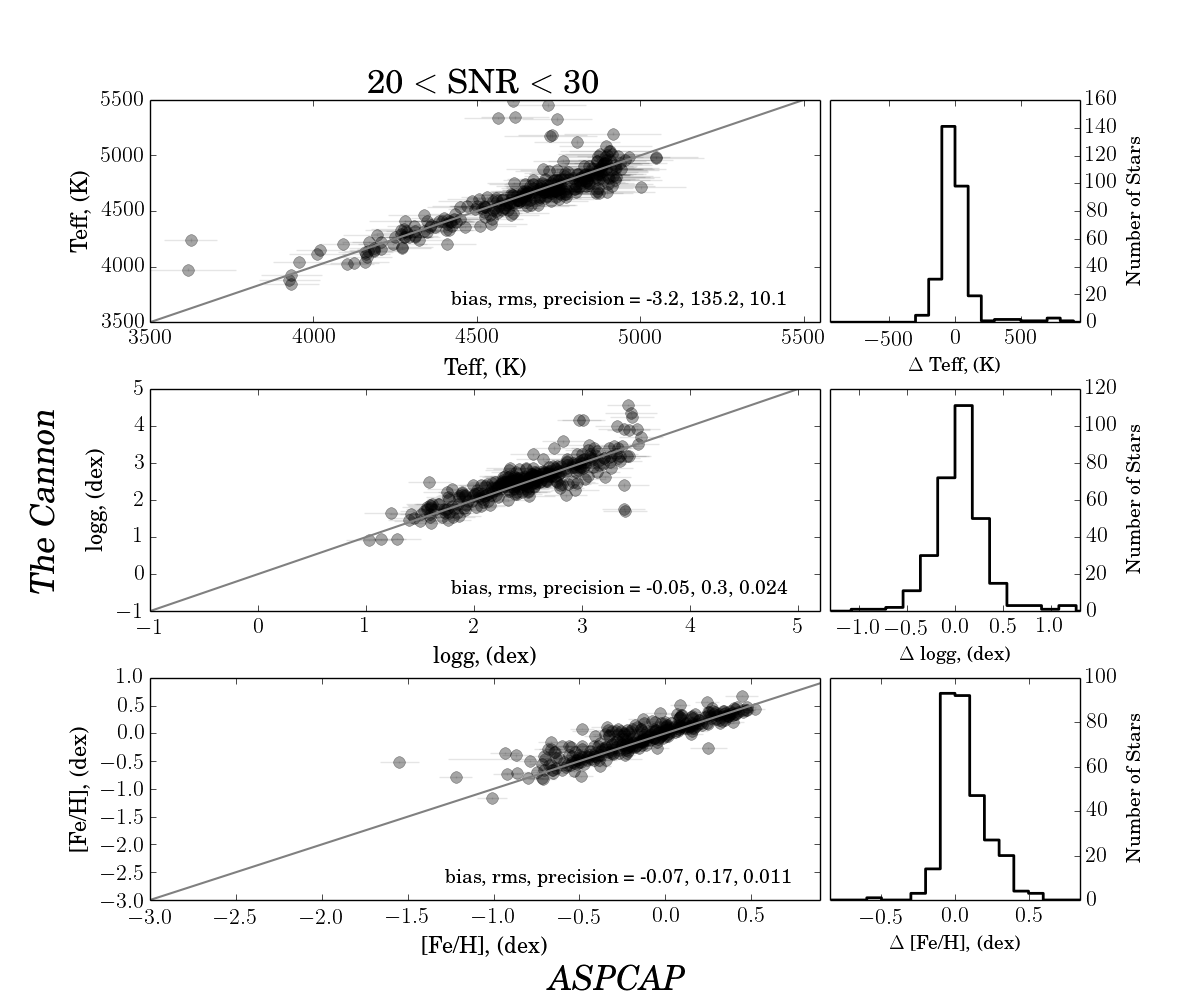
\includegraphics[scale=0.25]{./plots/SNR20to30.pdf}
    \caption{Four regimes of SNR for single visit spectra. There are 60 stars in the 300 $<$  SNR $<$ 30 bin, 1200 stars in the 30 $<$ SNR $<$ 50 bin, 1100 stars in the 50 $<$ SNR $<$ 100 bin and 670 stars in the 100 $<$  SNR $<$ 200 bin.}
\label{fig:SNR}
\end{figure}

 
 % run -i makecontin_data1_split.py


By identifying `true' continuum pixels we have been able to implement a simple continuum normalisation that is robust across low and high SNR, which is valid across the parameter range of our training set. To examine how \tc\ performs at lower SNR, we have taken individual visits from the apStar fits files, when there are $\ge$ 4 visits, and run \tc\ on a single visit spectra which we have continuum-normalised. Note, we have not simply noisifyed the combined visit data for our low SNR tests so this relies on both a robust continuum normalisation and the success of the label-transfer method. Figure \ref{fig:lowsnr} shows a comparison of a sample star for a single visit and combined visits ($>$ 4 total visits). Figure \ref{fig:SNR} presents the results of \tc\ compared to \apogee\ for these stars, showing \textit{only} the \apogee\ stars with errors of $<$ 150 K in \teff\ and $<$ 0.25 dex in \logg, across four SNR intervals, from 20 $<$ SNR $<$ 30 to 100 $<$ SNR $<$ 200. 



These Figures illustrate that the continuum normalisation works well for both of these SNR regimes and is SNR independent, which is not true for a weighted-quantile normalisation. At the highest SNR (and \apogee\ estimates a upper noise floor of 200 although stars do measure above this), the rms difference between \tc\ and \aspcap\ is comparable to the \aspcap\ measurement errors, at 73K in \teff\, 0.18 dex in \logg\ and 0.11 dex in \feh.  At a SNR of 30-50, the rms error increases to 100 K, 0.2 dex and 0.10 dex in \teff, \logg\ and \feh\, respectively. At an SNR of 20-30 the rms error is significantly higher and here the internal errors of \tc\ become comparable to typical minimisation methods and at SNR $<$ 20 exceed them. With this method we can return stellar parameters of \teff, \logg, \feh\ to as good a precisions as minimisation techniques ( \teff\ $<$ 100K, \logg\ $<$ 0.2 dex, \feh\ $< $0.1 dex) with an SNR of $\ge$ 25. 
 



\section{Discussion}

We have demonstrated in \tc,  that label-transfer is possible and extremely successful to determine stellar parameters in large surveys, simply and efficiently. This approach argues for defined stellar standards to effectively transfer labels of benchmark stars, studied at high resolution, to stars in surveys across any wavelength region. This would enable all stellar surveys to be unified. 

We have  proven how models in the optical, which must be explicitly used to define the labels for the benchmark stars,  can be effectively used in the infrared via this transfer. Furthermore, using a data-driven model, we then do not rely on explicit models in a new wavelength region of analysis. In this way we can fully capitalise on large surveys and the information in the data itself and not be penalised by simplified stellar models and uncertainties in linelists in new regions. 

We reproduce the \apogee\ labels without adding any significant uncertainty because we use every pixel in the spectra and let the noise model determine the weighting of the luminosity function, yet we can only do better. We have also demonstrated that we can work at much lower SNR at least for the three primary stellar parameters. We expect to not gain the same advantage for individual elements, but it may be possible to combine elements into subgroups (e.g. alpha light elements, neutron capture) of covariant spaces (e.g. Ting et al., 2012) and so exploit more pixels in the spectra and operate at significantly lower signal to noise without being penalised in dimensionality of the returned parameter and abundance space. 

data driven model -  very successful as it respects the noise model. generative - synth, L.F. - permits discovery, interpretation.

We have barely scratched the surface with what is possible with this methodology and our training set, model and labels are very restricted. Our training data set itself is clearly too small, comprising only 500 stars including a set of dwarfs at a single metallicity (+0.03 dex). As we lack dwarfs in particular we can not return parameters in this space to the same precision as giants (\logg\ $\le$ 3.5).  We also are missing any dwarfs with rotation in our model and consequently these are returned in an unphysical \teff-\logg\ parameter space in the label-transfer. We also assume our training set is absolute, we do not include any errors in our adopted labels, which reduces the flexibility of our model and is not correct.We currently treat every pixel as independent which is incorrect and therefore an incomplete model, missing the real physical representation. Nevertheless, we have shown using the APOGEE data that even the simplest model with naive assumptions and an incomplete physical description, works. This method is directly transferrable as is, to all other surveys and we expect we would be similarly successful applying this to e.g. \textit{GALAH} and \gaiaeso.



\tc\ is readily expandable to a more general model, a larger training set and many more labels, and relevant for chemical tagging. 
Our second-order model is hard coded and extremely restrictive and this can be upgraded to a Gaussian process and include assumptions of priors as currently there is no use of any prior physical knowledge in our model. It is also possible to implement exactly the same procedure we describe using a synthetic grid instead of data to create the model and this will remove many of these limitations in the model. However, this also convolve in unphysical representations of stars as stellar models are simplified versions of real data. We preferably argue for adopting a wider set of benchmark stars from data in surveys, given labels determined at high resolution. 

We identify new opportunities with this approach. The primary and obvious opportunity is to unify all stellar parameter systems and a key necessity of this is that all common benchmark stars be observed in all surveys. The data driven model itself also enables an analysis and characterisation of how and where stellar templates diverge from data. Using the coefficients of the labels returned in this method, we can also directly identify and learn where the information in a stellar spectrum resides and make quantitative assessments of the flux dependence on the labels and for example determine continuum pixels. The information in the spectra itself is a direct output from the model, which is more general and immensely more informative than the reverse assumption of assessing regions of interest as informed by linelists.  A direct first additional upgrade for \tc\ is  to add more labels and an obvious initial choice is $\alpha$-enhancement, followed by individual abundances [X/Fe]. It is even possible to test what, if any information is contained in labels such as age. If such information is present in the spectra across a large set of stars in a survey, this method will determine exactly which pixels are responsible for carrying this information. In addition, we will gain significantly by moving to a more flexible model like a Gaussian process and allowing our model to be informed by priors.

As \tc\ is a way to understand the spectra, it is highly relevant for chemical tagging where simple determination of individual elemental abundances and analysis of grouping across this parameter space will unlikely suffice. Conversely, a direct differential analysis of the data is a powerful approach using the data itself, without simplified assumptions in models. 

From our implementation of \tc\ on APOGEE data, we were motivated to examine the calibration space of the labels given the unphysically narrow giant branch returned for DR10 data at low \logg. We found by adopting a calibration that shifts the stars to the nearest position on the isochrone (keeping the \teff\ and \feh\ fixed to \aspcap\ corrected values), the stars shifted onto the isochrones in \teff-\logg\ space, across metallicity, in line with expectations of the physical parameter space of stars. This small \logg\ adjustment is naive, but works well, causing small shifts in the \logg\ scale at low temperatures compared to the \apogee\ \logg\ input labels. This suggests that there is some problem with the input labels in the \logg\ dimension adjusted from Kepler results in DR10. 

\textbf{ $\bullet$  DWH add your discussion here?} 

%The future iteration of \tc\ will be to implement a gaussian process, bringing in errors and we can training on individual labels from DR12 to see if can reproduce individual labels in the rest of DR12 data given these labels in the training spectra, via the label-transfer. Will not be a function of synthetic spectra as data driven model. 

%Data-driven models carry physically correct details that will be missing from synthetic stelar models which make simplified assumptions about stellar physics.  and the agreement with Kepler \logg\ values was also found to be good

% add references!!

\acknowledgements{DFM primary, 
JB, sloan
DWH grant no.,
The research has
received funding from the European Research Council under the European
Union's Seventh Framework Programme (FP 7) ERC Grant Agreement n.
[321035]. MA acknowledges generous funding from the Australian Research Council (grant FL110100012)\\

Funding for SDSS-III has been provided by the Alfred P. Sloan Foundation, the Participating Institutions, the National Science Foundation, and the U.S. Department of Energy Office of Science. The SDSS-III web site is $http://www.sdss3.org/.$\\

SDSS-III is managed by the Astrophysical Research Consortium for the Participating Institutions of the SDSS-III Collaboration including the University of Arizona, the Brazilian Participation Group, Brookhaven National Laboratory, Carnegie Mellon University, University of Florida, the French Participation Group, the German Participation Group, Harvard University, the Instituto de Astrofisica de Canarias, the Michigan State/Notre Dame/JINA Participation Group, Johns Hopkins University, Lawrence Berkeley National Laboratory, Max Planck Institute for Astrophysics, Max Planck Institute for Extraterrestrial Physics, New Mexico State University, New York University, Ohio State University, Pennsylvania State University, University of Portsmouth, Princeton University, the Spanish Participation Group, University of Tokyo, University of Utah, Vanderbilt University, University of Virginia, University of Washington, and Yale University.\\

}

\end{document}
